\documentclass[11pt, reqno, letterpaper, twoside]{amsart}
\linespread{1.2}
\usepackage[margin=1.25in]{geometry}

\usepackage{amssymb, bm, mathtools, physics}
\usepackage[dvipsnames,svgnames,table]{xcolor} % 移除 usenames
\usepackage{graphicx} % 移除 [pdftex, xetex]
\usepackage{enumerate, setspace}
\usepackage{float, colortbl, tabularx, longtable, multirow, subcaption, environ, wrapfig, textcomp, booktabs}
\usepackage{pgf, tikz, framed}
\usepackage[normalem]{ulem}
\usetikzlibrary{arrows,positioning,automata,shadows,fit,shapes}
\usepackage[english]{babel}
\usepackage{listings}
\usepackage[final]{microtype}

\lstset{
    language=Python,                % 语言
    basicstyle=\ttfamily\small,     % 字体
    keywordstyle=\color{blue},      % 关键字颜色
    commentstyle=\color{green!50!black}, % 注释颜色
    stringstyle=\color{red},        % 字符串颜色
    showstringspaces=false,         % 不显示空格
    frame=single,                   % 外框
    breaklines=true                 % 自动换行
}

\theoremstyle{plain}
\newtheorem{theorem}{Theorem}

\theoremstyle{definition}
\newtheorem{solution}[theorem]{Solution}

\usepackage{times}

\title{ESE 546\\[0.1in]
Homework 1}
\author{
Jinhao You [you7@seas.upenn.edu]
}



\begin{document}
\maketitle

\begin{solution}[Time spent: 5 hours]
Your solution goes here.
\\One possib;le objective function chould be this type shown below:
\paragraph{Problem a}
    \begin{equation*}
    \begin{aligned}
    \min_{w,\,b,\,\xi} \quad & \frac{1}{2}\lVert w \rVert^2 
        + C \sum_{i=1}^{n} \xi_i \\
    \text{s.t.} \quad & y_i \big( w^\top x_i + b \big) \geq 1 - \xi_i, \quad i=1,\dots,n, \\
    & \xi_i \geq 0, \quad i=1,\dots,n .
    \end{aligned}
    \end{equation*}
\end{solution}

\paragraph{Problem b}
    In SVM, \textbf{support samples} are those training samples that lie exactly on the margin boundary, 
    satisfying the equality constraint:
    \[
    y_i \big( \theta^\top x_i + \theta_0 \big) = 1 .
    \]

\paragraph{Problem c}
I executed the code below to verify that the dataset was downloaded correctly. 
The output displays a random image from the MNIST dataset, confirming the success of the download process.
\begin{figure}[H]
    \centering
    \begin{subfigure}[b]{0.5\textwidth}
        \centering
        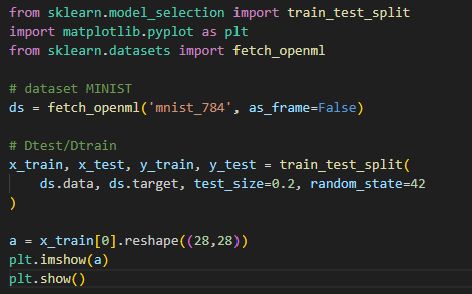
\includegraphics[width=\textwidth]{image/prob1_c_1.png}
        \caption{Code for downsampling}
        \label{fig:first}
    \end{subfigure}
    \hfill
    \begin{subfigure}[b]{0.4\textwidth}
        \centering
        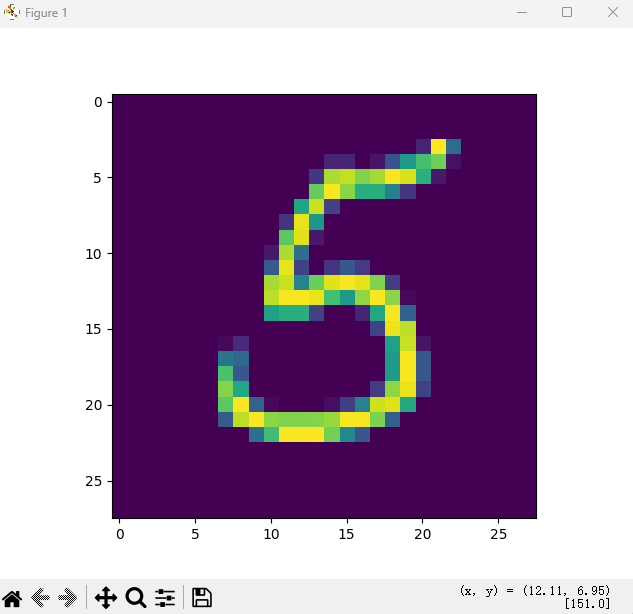
\includegraphics[width=\textwidth]{image/prob1_c_1.1.png}
        \caption{Random image from MINIST after downsampling}
        \label{fig:second}
    \end{subfigure}
    
    \caption{Downsampling process and results.}
    \label{fig:twopics}
\end{figure}

For the downsampling step (from $28 \times 28$ to $14 \times 14$), the \textit{cv2} library was employed. 
The procedure and the corresponding results are presented below:
\begin{figure}[H]
    \centering
    \begin{subfigure}[b]{0.5\textwidth}
        \centering
        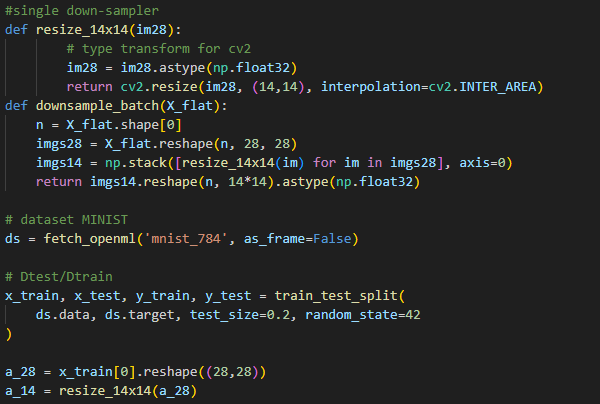
\includegraphics[width=\textwidth]{image/prob1_c_2.png}
        \caption{Code for downloading}
        \label{fig:first}
    \end{subfigure}
    \hfill
    \begin{subfigure}[b]{0.4\textwidth}
        \centering
        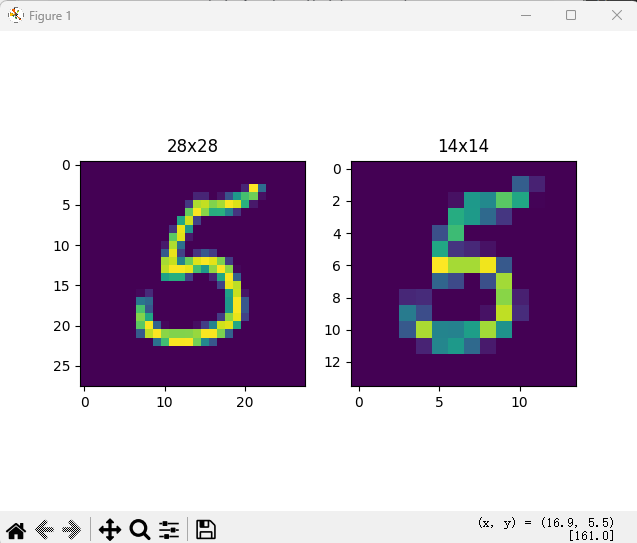
\includegraphics[width=\textwidth]{image/prob1_c_2.1.png}
        \caption{Random image from MINIST}
        \label{fig:second}
    \end{subfigure}
    
    \caption{Dataset download and random image from the dataset.}
    \label{fig:twopics}
\end{figure}

\paragraph{\textbf{Problem d}}
The parameter $C$ controls the trade-off between maximizing the margin and minimizing the classification error on the training data. 
A larger value of $C$ places more emphasis on correctly classifying all training examples (risking overfitting), 
whereas a smaller value of $C$ encourages a wider margin at the cost of allowing more misclassifications (potentially improving generalization). 
The parameter $\gamma$ (in the RBF kernel) determines the influence of a single training example. 
A small value of $\gamma$ results in a smoother decision boundary, while a large value of $\gamma$ 
leads to a more complex boundary that may overfit the training data. 
By default, in \texttt{scikit-learn}, $C=1.0$ and $\gamma='scale'$.

Figures below show how the training process was conducted and the corresponding results with set $\gamma='auto'$. 
\begin{figure}[H]
    \centering
    \begin{subfigure}[b]{0.5\textwidth}
        \centering
        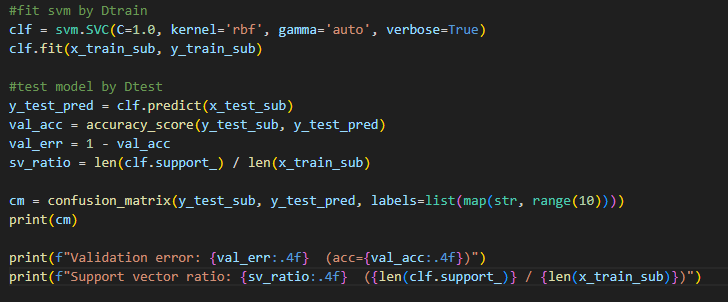
\includegraphics[width=\textwidth]{image/prob1_d_1.png}
        \caption{Code for fitting}
        \label{fig:first}
    \end{subfigure}
    \hfill
    \begin{subfigure}[b]{0.4\textwidth}
        \centering
        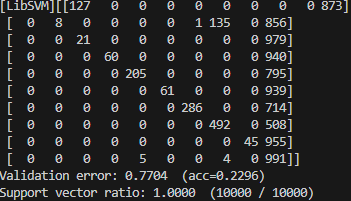
\includegraphics[width=\textwidth]{image/prob1_d_1.1.png}
        \caption{Results with  $\gamma='auto'$}
        \label{fig:second}
    \end{subfigure}
    
    \caption{SVM fitting and the results.}
    \label{fig:twopics}
\end{figure}

After fitting the SVM classifier on the training data, the validation error was found to be 
77.04\%. The ratio of support vectors to the total number of training samples is 
100\%, which indicates all samples were critical in defining the decision boundary. The confusion matrix on the test set is shown below:

\[
\begin{bmatrix}
127 & 0 & 0 & 0 & 0 & 0 & 0 & 0 & 0 & 873 \\
8 & 0 & 0 & 0 & 0 & 1 & 135 & 0 & 0 & 856 \\
0 & 21 & 0 & 0 & 0 & 0 & 0 & 0 & 0 & 979 \\
0 & 0 & 60 & 0 & 0 & 0 & 0 & 0 & 0 & 940 \\
0 & 0 & 0 & 205 & 0 & 0 & 0 & 0 & 0 & 795 \\
0 & 0 & 0 & 0 & 61 & 0 & 0 & 0 & 0 & 939 \\
0 & 0 & 0 & 0 & 0 & 286 & 0 & 0 & 0 & 714 \\
0 & 0 & 0 & 0 & 0 & 0 & 492 & 0 & 0 & 508 \\
0 & 0 & 0 & 0 & 0 & 0 & 0 & 45 & 0 & 955 \\
0 & 0 & 0 & 0 & 0 & 0 & 0 & 0 & 4 & 991
\end{bmatrix}
\]

From the matrix, it is clear that most samples were misclassified as class ``9''. 
For instance, digits such as ``0'', ``1'', and ``4'' were predominantly confused with ``9''. 
This suggests that the classifier failed to construct meaningful decision boundaries 
and instead assigned most inputs to a single class. 
Intuitively, this poor performance can be attributed to the choice of the kernel parameter $\gamma$. 
Specifically, the model was trained with \texttt{gamma="auto"} instead of the recommended \texttt{gamma="scale"}. 
When \texttt{gamma="auto"} is used, $\gamma$ is set to $1/n_{\text{features}}$, which is often too small for high-dimensional data such as MNIST. 
This results in a nearly linear decision boundary that fails to capture the data distribution, 
leading to all samples being treated as support vectors and the classifier collapsing to predict almost exclusively one class. 
In contrast, the default setting \texttt{gamma="scale"} adjusts $\gamma$ based on both the number of features and the variance of the data, 
and typically yields significantly better generalization.

When training the SVM with $\gamma=\texttt{"scale"}$, the model achieved a validation error of 
3.97\% . The ratio of support vectors was 34.88\%, which indicates that 
only about one-third of the training samples were critical in defining the decision boundary, 
showing that the classifier generalized much better compared to the \texttt{"auto"} setting.

The confusion matrix on the test set is as follows:
\[
\begin{bmatrix}
982 & 0 & 4 & 0 & 1 & 1 & 4 & 1 & 5 & 2 \\
0 & 988 & 2 & 3 & 1 & 0 & 3 & 2 & 0 & 1 \\
5 & 4 & 956 & 6 & 2 & 6 & 5 & 7 & 7 & 1 \\
1 & 4 & 14 & 939 & 0 & 20 & 2 & 5 & 10 & 5 \\
2 & 1 & 6 & 0 & 965 & 0 & 7 & 1 & 1 & 17 \\
1 & 3 & 1 & 15 & 3 & 962 & 7 & 0 & 6 & 0 \\
1 & 0 & 0 & 6 & 9 & 0 & 982 & 0 & 2 & 0 \\
0 & 7 & 9 & 2 & 6 & 0 & 9 & 959 & 2 & 15 \\
2 & 2 & 6 & 13 & 5 & 10 & 8 & 9 & 930 & 31 \\
4 & 7 & 11 & 11 & 19 & 2 & 0 & 12 & 4 & 940
\end{bmatrix}
\]

From the matrix, I observe that most predictions are correct along the diagonal, 
with only minor confusions. For example, some ``4'' digits are misclassified as ``9'', 
and some ``8'' digits are confused with ``9'' or ``3''. These errors are intuitive, 
as the corresponding digits share similar shapes and strokes. 
Overall, the classifier trained with $\gamma=\texttt{"scale"}$ shows strong generalization 
and performs significantly better than the model trained with $\gamma=\texttt{"auto"}$.

Using $\gamma=\texttt{"scale"}$, the SVM classifier was evaluated on the full test set. 
The model achieved a test error of 3.99\%, 
with a support vector ratio of 34.88\%. 
This indicates that only about one-third of the training samples were critical support vectors, 
confirming that the classifier generalized well.

The confusion matrix on the full test data is given by:
\[
\begin{bmatrix}
1319 & 1 & 5 & 0 & 1 & 2 & 5 & 1 & 7 & 2 \\
0 & 1578 & 3 & 8 & 1 & 0 & 1 & 4 & 4 & 1 \\
5 & 9 & 1318 & 7 & 5 & 7 & 9 & 10 & 8 & 2 \\
1 & 6 & 17 & 1345 & 1 & 28 & 4 & 10 & 14 & 7 \\
2 & 1 & 6 & 0 & 1246 & 0 & 7 & 2 & 1 & 30 \\
3 & 4 & 2 & 21 & 3 & 1224 & 10 & 2 & 6 & 0 \\
1 & 10 & 12 & 2 & 9 & 0 & 1440 & 2 & 2 & 27 \\
3 & 12 & 9 & 18 & 11 & 23 & 11 & 1261 & 6 & 3 \\
6 & 9 & 1 & 15 & 23 & 4 & 0 & 19 & 6 & 1337
\end{bmatrix}
\]

The diagonal dominance of the matrix shows that most digits are correctly classified. 
The misclassifications are sparse and primarily involve visually similar digits, 
such as ``4'' being confused with ``9'' and ``8'' with ``3''. 
These mistakes are intuitive, as such digit pairs share structural similarities. 

Overall, the results on the full test set confirm the strong generalization performance of the SVM with $\gamma=\texttt{"scale"}$, 
which performs significantly better than the $\gamma=\texttt{"auto"}$ setting.

\paragraph{Problem e}
The \texttt{sklearn.svm.SVC} class exposes several options beyond the basic SVM formulation, 
including parameters such as C, kernel, degree, gamma, 
 \texttt{shrinking}. Many of these are not part of the “vanilla” SVM theory, 
but are provided in practice to improve performance and usability.

The parameter shrinking controls whether the shrinking 
heuristic is applied during optimization. Shrinking heuristics temporarily remove variables 
(dual coefficients) that are unlikely to change from the optimization problem, 
thereby reducing the problem size and speeding up convergence. 
In practice, enabling shrinking often leads to faster training without affecting the final solution.

Scikit-learn's SVCis built on top of LIBSVM. 
Thus, the optimization algorithm it uses is the Sequential Minimal Optimization (SMO) method, 
which decomposes the quadratic programming problem into smaller subproblems involving 
only two Lagrange multipliers at a time, making the optimization efficient and scalable.\\

\paragraph{Problem f}
By default, svm.SVC in scikit-learn calls LIBSVM, which uses the one-vs-one (OvO) strategy 
for handling multi-class problems. For a K-class classification task, this requires training 
$\tfrac{K(K-1)}{2}$ binary classifiers. For example, with K=10 classes (as in MNIST), 
45 binary classifiers are trained. At prediction time, each binary classifier casts a vote, 
and the final label is chosen by majority voting.

Other common extensions of binary classification to the multi-class setting include:
One-vs-Rest (OvR) with each classifier distinguishes whether a sample belongs to class k versus "not k". 
For K classes, K classifiers are trained. At test time, all classifiers are evaluated, 
and the class with the highest confidence score is chosen.

Error-Correcting Output Codes (ECOC) with each class is assigned a codeword, for example a binary string. 
Training is performed for each bit position of the codeword, resulting in multiple binary classifiers. 
At prediction time, the predicted codeword is compared with all class codewords, 
and the nearest one is selected. This provides robustness against individual classifier errors.\\

\paragraph{Problem g}
I tuned the penalty parameter C using \texttt{sklearn.model\_selection.GridSearchCV} on the training split, 
keeping kernel = rbf and gamma = "scale". I evaluated at 11 candidates for C and report the
cross-validated mean accuracy together with the validation accuracy computed on the held-out validation set.

\begin{enumerate}
  \item Parameter grid: C in \{[0.1, 0.5, 1.5, 2.5, 3, 3.5, 4, 4.5, 5, 5.5, 6]\}.
  \item Inner cross-validation: k-fold CV (k = [5]) within GridSearchCV on the training split.
  \item Model selection: choose the C with the highest validation accuracy; if there is a tie, prefer the smaller C.
\end{enumerate}


Figures below show how to find best parameter by using GridsearchCV with k=5.
\begin{figure}[H]
    \centering
    \begin{subfigure}[b]{0.45\textwidth}
        \centering
        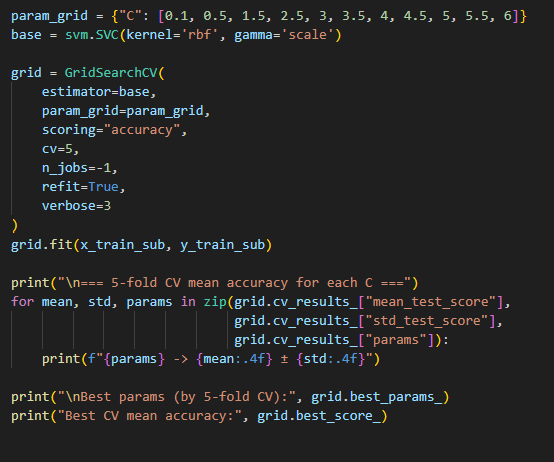
\includegraphics[width=\textwidth]{image/prob1_g_1.png}
        \caption{Code for GridsearchCV}
        \label{fig:first}
    \end{subfigure}
    \hfill
    \begin{subfigure}[b]{0.45\textwidth}
        \centering
        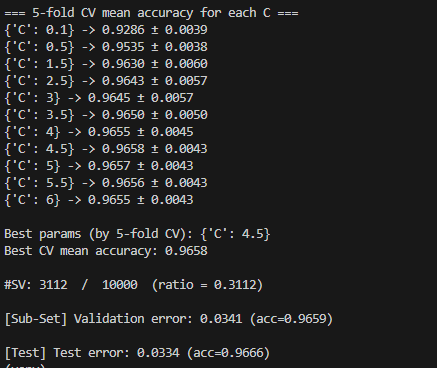
\includegraphics[width=\textwidth]{image/prob1_g_1.1.png}
        \caption{Results with  k = 5}
        \label{fig:second}
    \end{subfigure}
    
    \caption{Groups of results obtained by GridsearchCV}
    \label{fig:twopics}
\end{figure}

The best parameter selected by 5-fold cross validation was C = 4.5, with a mean accuracy of 96.58\%. 
The number of support vectors was 3112 out of 10000, giving a ratio of 31.13\%. 
On the held-out validation subset, the error rate was 34.10\%. 
On the full test set, the error rate was 33.40\%. 
These results show that the tuned model generalizes well and achieves slightly better performance than the default choice.\\

\paragraph{Problem h and j}
I applied the Gabor filter bank with multiple parameter settings for frequency, 
orientation angle, and bandwidth. The goal was to analyze how different filter 
configurations highlight various spatial features of the MNIST images and to use 
the resulting coefficients as input features for an SVM classifier. 

Before applided filter bank, I tested the filters consisting of the following parameter combinations
\begin{figure}[H]
    \centering
    % 第一行
    \begin{subfigure}[b]{0.45\textwidth}
        \centering
        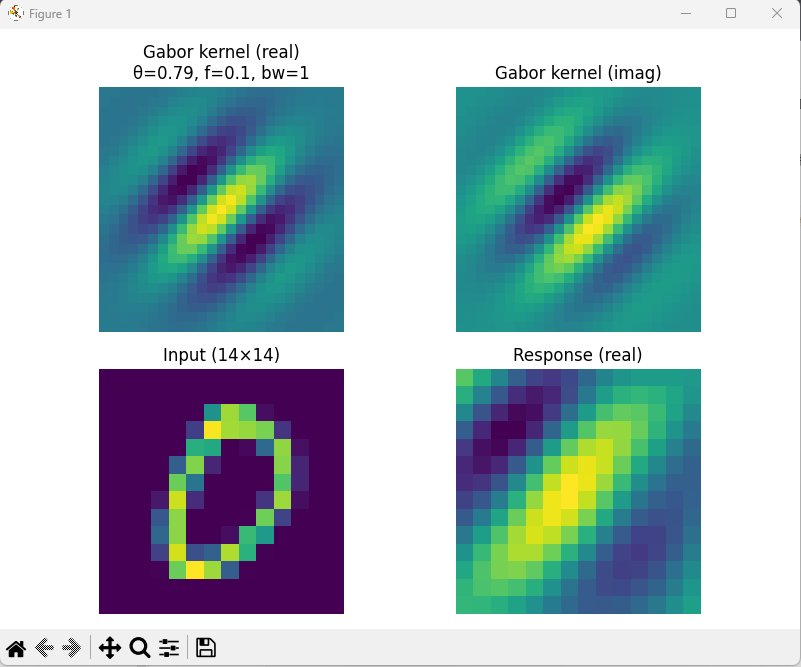
\includegraphics[width=\textwidth]{image/prob1_h_1.png}
        \caption{frequency=0.1, theta=$\pi/4$, bandwidth=0.6}
        \label{fig:gabor-1}
    \end{subfigure}\hfill
    \begin{subfigure}[b]{0.45\textwidth}
        \centering
        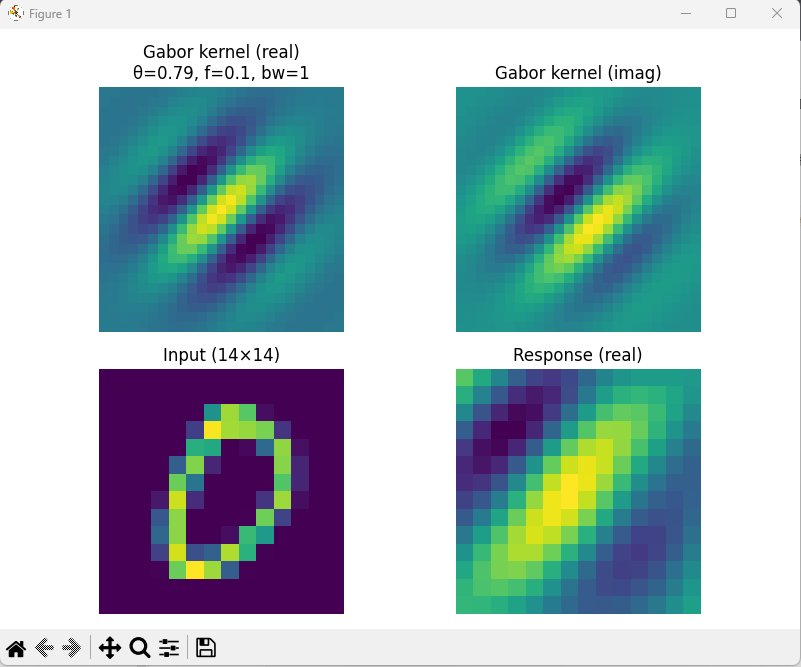
\includegraphics[width=\textwidth]{image/prob1_h_1.1.png}
        \caption{frequency=0.1, theta=$\pi/4$, bandwidth=1}
        \label{fig:gabor-2}
    \end{subfigure}

    % 第二行
    \begin{subfigure}[b]{0.45\textwidth}
        \centering
        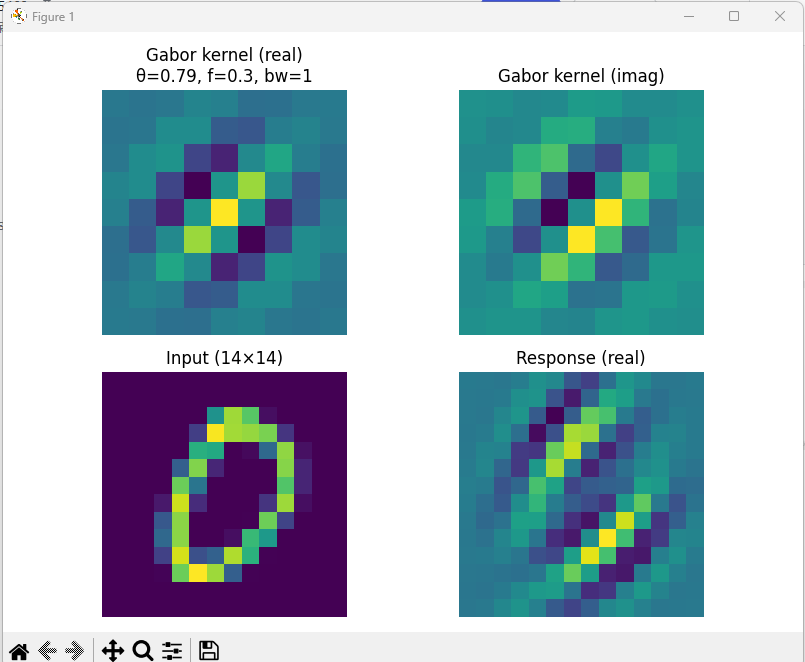
\includegraphics[width=\textwidth]{image/prob1_h_2.png}
        \caption{frequency=0.3, theta=$\pi/2$, bandwidth=0.6}
        \label{fig:gabor-3}
    \end{subfigure}\hfill
    \begin{subfigure}[b]{0.45\textwidth}
        \centering
        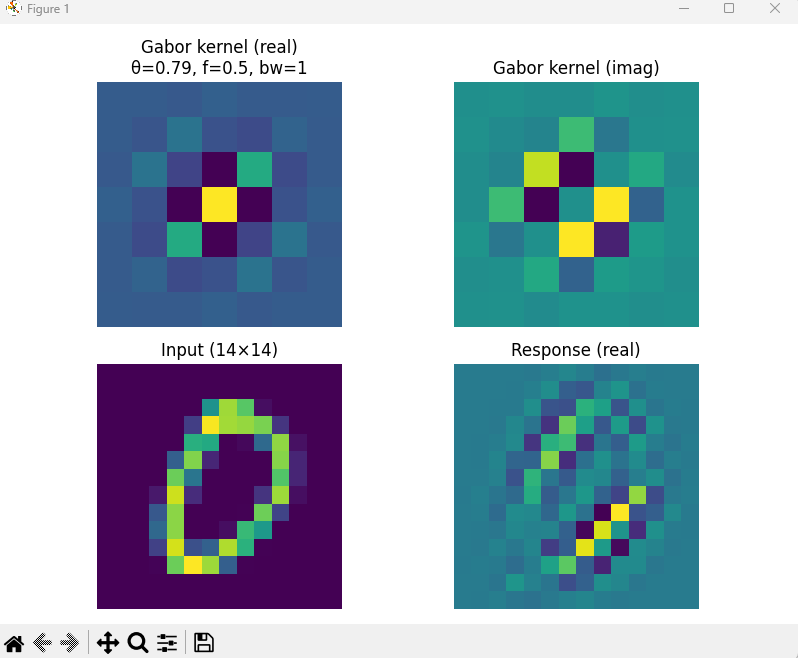
\includegraphics[width=\textwidth]{image/prob1_h_2.1.png}
        \caption{frequency=0.5, theta=$\pi$, bandwidth=1}
        \label{fig:gabor-4}
    \end{subfigure}

    % 第三行
    \begin{subfigure}[b]{0.45\textwidth}
        \centering
        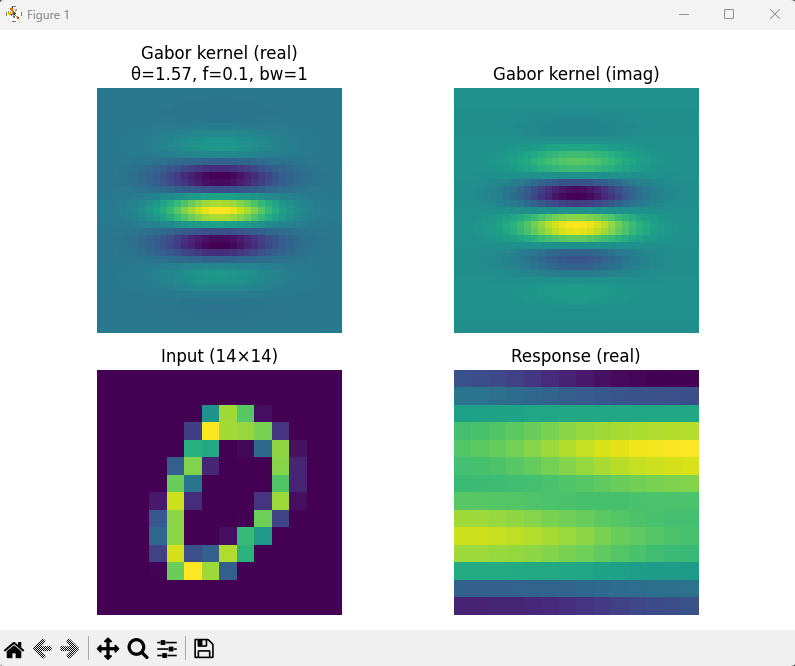
\includegraphics[width=\textwidth]{image/prob1_h_3.png}
        \caption{frequency=0.1, theta=$\pi/4$, bandwidth=0.6}
        \label{fig:gabor-5}
    \end{subfigure}\hfill
    \begin{subfigure}[b]{0.45\textwidth}
        \centering
        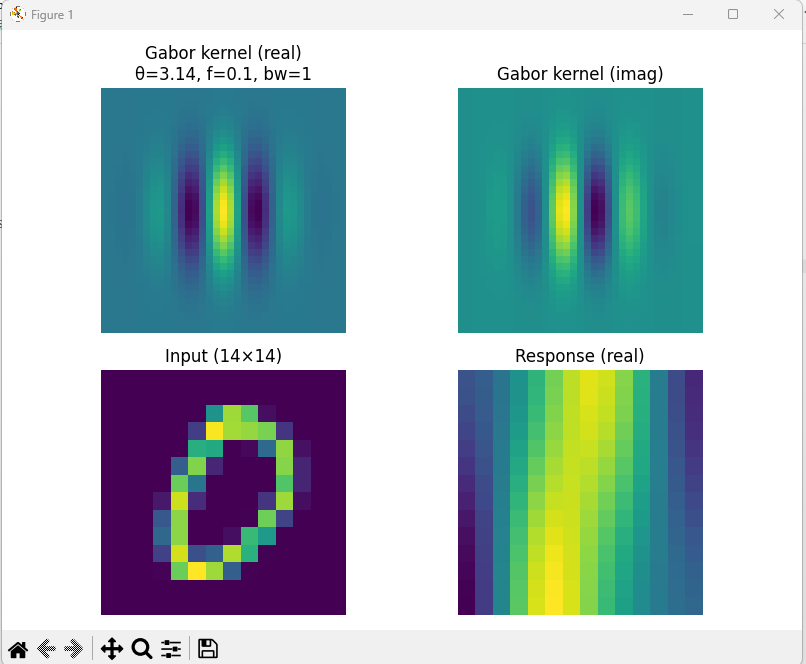
\includegraphics[width=\textwidth]{image/prob1_h_3.1.png}
        \caption{frequency=0.1, theta=$\pi/4$, bandwidth=1}
        \label{fig:gabor-6}
    \end{subfigure}

    \caption{Groups of results obtained by Gabor filters with different parameters}
    \label{fig:gabor-all}
\end{figure}

Then I constructed a Gabor filter bank with 36 filters and applied it to each downsampled image of size
$14 \times 14 = 196$ pixels. Concatenating the responses from all filters yields a feature vector of length
$196 \times 36 = 7056$ per image.

\begin{figure}[H]
    \centering
    % 第一张
    \begin{subfigure}[b]{0.32\textwidth}
        \centering
        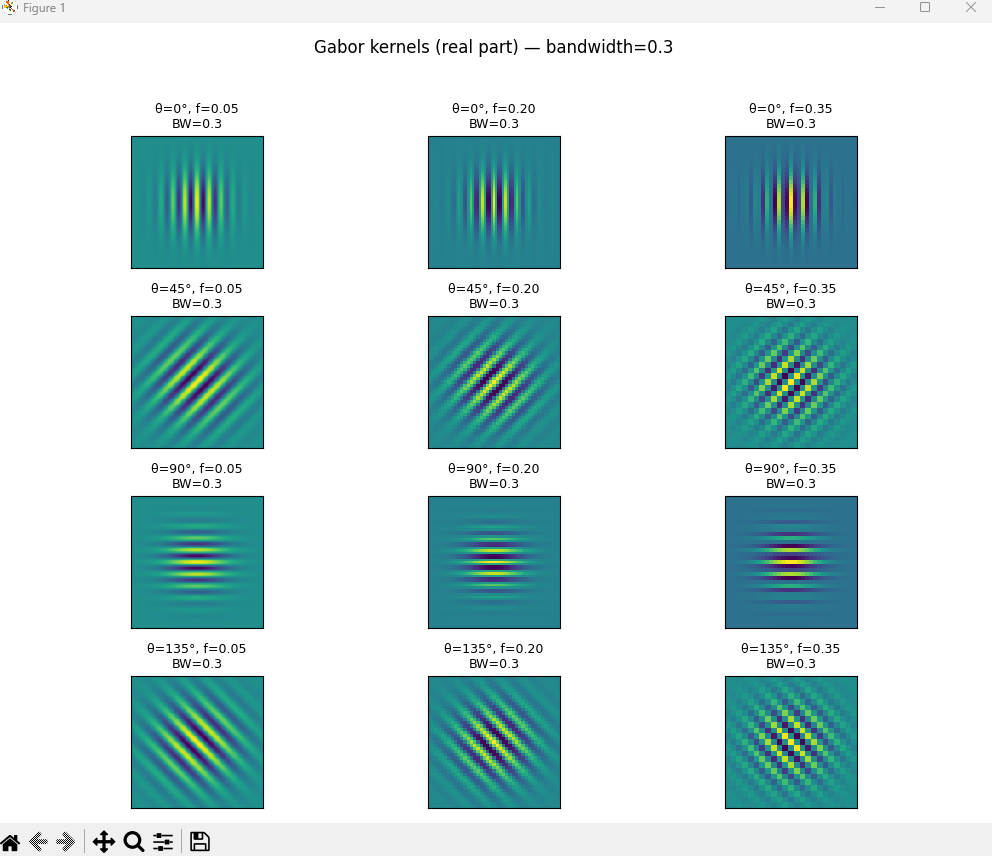
\includegraphics[width=\textwidth]{image/prob1_j_1.png}
        \caption{}
        \label{fig:three-1}
    \end{subfigure}
    % 第二张
    \begin{subfigure}[b]{0.32\textwidth}
        \centering
        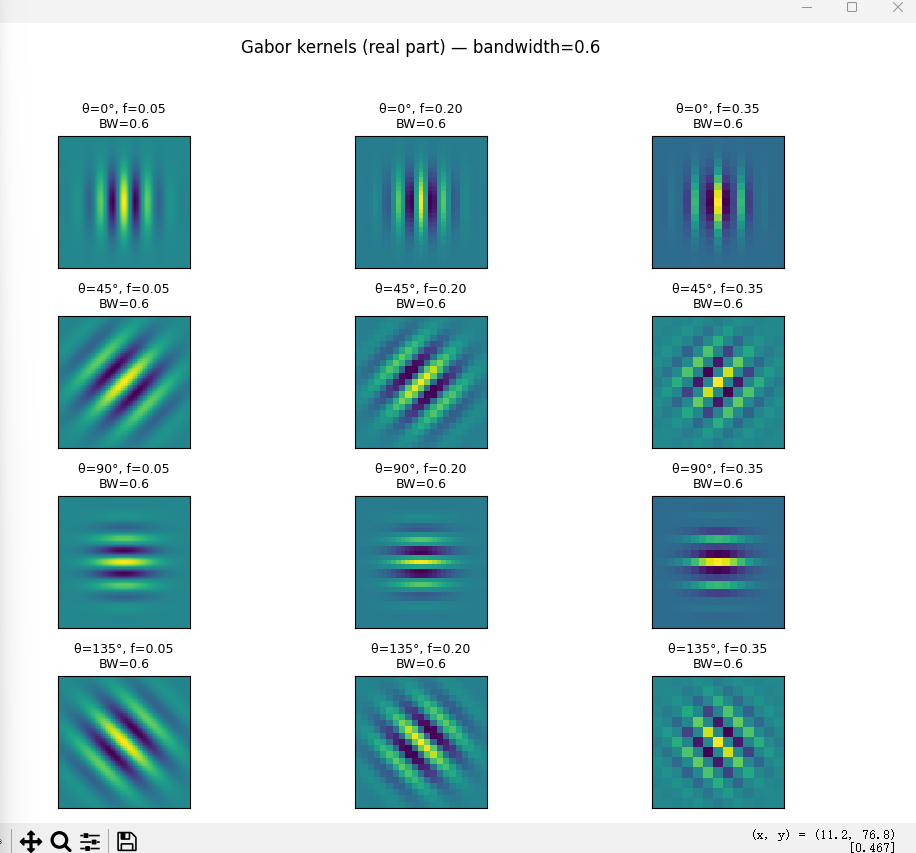
\includegraphics[width=\textwidth]{image/prob1_j_1.1.png}
        \caption{}
        \label{fig:three-2}
    \end{subfigure}
    % 第三张
    \begin{subfigure}[b]{0.32\textwidth}
        \centering
        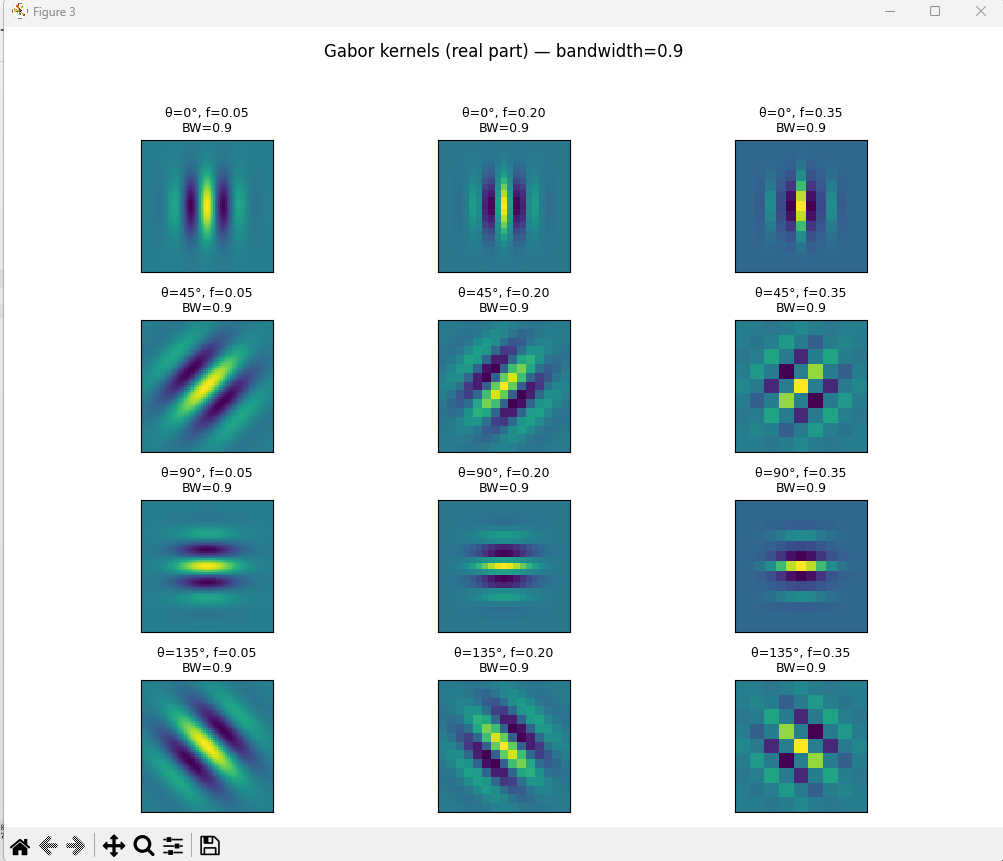
\includegraphics[width=\textwidth]{image/prob1_j_1.2.png}
        \caption{}
        \label{fig:three-3}
    \end{subfigure}

    \caption{Visualization of the 36-filter bank covering multiple orientations and frequencies.}
    \label{fig:three-all}
\end{figure}

I trained an SVM with RBF kernel on these features and evaluated performance on the training and validation splits.

\begin{table}[H]
\centering
\begin{tabular}{lccc}
\hline
Setting & Train accuracy &  Support vector ratio \\
\hline
36 filters (no PCA) & [90.60\%]  & [64.80\%] \\
\hline
\end{tabular}
\caption{Baseline results using the 36-filter bank.}
\label{tab:baseline-36}
\end{table}

Next, I increased the number of filters to obtain a denser coverage of orientations and scales. Since the
feature dimensionality grows linearly with the number of filters, I applied PCA to reduce dimensionality
before training the SVM. I evaluated the performance of an SVM classifier trained on features extracted 
from a 144-filter Gabor filter bank, using PCA to reduce dimensionality. 
Since the training set contained only 1000 samples, the maximum number of PCA 
components was limited to 999. This constraint restricted the effective 
dimensionality reduction and limited the classifier performance.

\begin{table}[H]
\centering
\begin{tabular}{lcccc}
\hline
Setting  & PCA components &  Test accuracy  &  Support vector ratio\\
\hline
144 filters   & [31] & [29.70\%] & [100\%]\\
144 filters   & [512] &  [44.80\%] &  [100\%]\\
144 filters   & [999] &  [81.90\%]  &  [100\%]\\
144 filters  + Standarlization& [999] &  [92.90\%]  &  [77.40\%]\\
\hline
\end{tabular}
\caption{Results after increasing the number of filters and applying PCA.}
\label{tab:pca-results}
\end{table}

As shown in the table, the classifier accuracy improves steadily as the number of 
PCA components increases, from 29.70\% with 31 components to 81.90\% with 999 
components. However, all models without feature standardization relied on all 
training samples as support vectors, indicating poor generalization. After applying 
standardization before SVM training, the accuracy increased further to 92.90\%, and 
the support vector ratio dropped to 77.40\%. This indicates that normalization of 
features is essential for stable training and improved generalization.

The overall limitation is that, with only 1000 training samples, PCA can produce 
at most 999 components. This prevented us from fully capturing the variance in 
the 7056-dimensional feature space produced by the 144 filters, and likely 
contributed to the performance gap compared to models trained with more data.

\clearpage
\begin{solution}[Time spent: 0.3 hour]
Your solution goes here.\\
\paragraph{Proof.}
For a convex differentiable function $\varphi$, every tangent is a global underestimator:
\[
\varphi(y) \;\geq\; \varphi(\mu) + \varphi'(\mu)\,(y-\mu) \quad \text{for all } y.
\]

Apply this inequality with $y = X$ and take expectations:
\[
\mathbb{E}[\varphi(X)] 
\;\geq\; \varphi(\mu) + \varphi'(\mu)\,\mathbb{E}[X-\mu]
\;=\; \varphi(\mu),
\]
since $\mathbb{E}[X-\mu] = 0$.


For geometric content of Jensen's inequality, a convex differentiable function, the tangent line at any point lies below the curve globally. 
At $\mu = \mathbb{E}[X]$, the tangent at $(\mu, \varphi(\mu))$ underestimates $\varphi(y)$ for all $y$. 
When I replace $y$ by the random variable $X$ and take expectations, the linear part of the tangent vanishes 
because $\mathbb{E}[X-\mu] = 0$. What remains is exactly $\varphi(\mu)$, showing that the function evaluated 
at the mean lies below the expected function value:
\[
\varphi(\mathbb{E}[X]) \;\leq\; \mathbb{E}[\varphi(X)].
\]

\end{solution}

\clearpage
\begin{solution}[Time spent: 5 hour]
Your solution goes here.\\
\paragraph{Problem a} We successfully downloaded the MNIST dataset using the provided code. The full training set 
contains 60,000 images and the validation set contains 10,000 images, both balanced across 10 classes. 
Following the instructions, we created a reduced dataset by taking 50\% of the samples from each class, 
resulting in about 30,000 training images and 5,000 validation images.

To verify that the dataset is correctly loaded and labeled, we plotted a few randomly selected images 
along with their corresponding labels. The examples below show digits that match their labels, confirming 
that the dataset is intact.

\begin{figure}[H]
    \centering
    \begin{subfigure}[b]{0.45\textwidth}
        \centering
        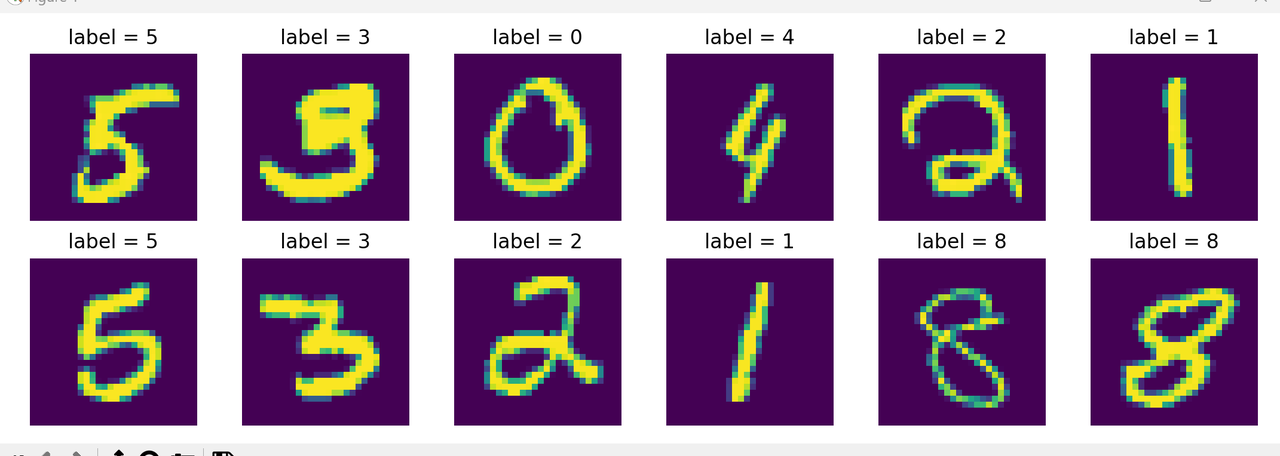
\includegraphics[width=\textwidth]{image/prob3_a_1_1.png}
        \caption{}
        \label{fig:first}
    \end{subfigure}
    \hfill
    \begin{subfigure}[b]{0.45\textwidth}
        \centering
        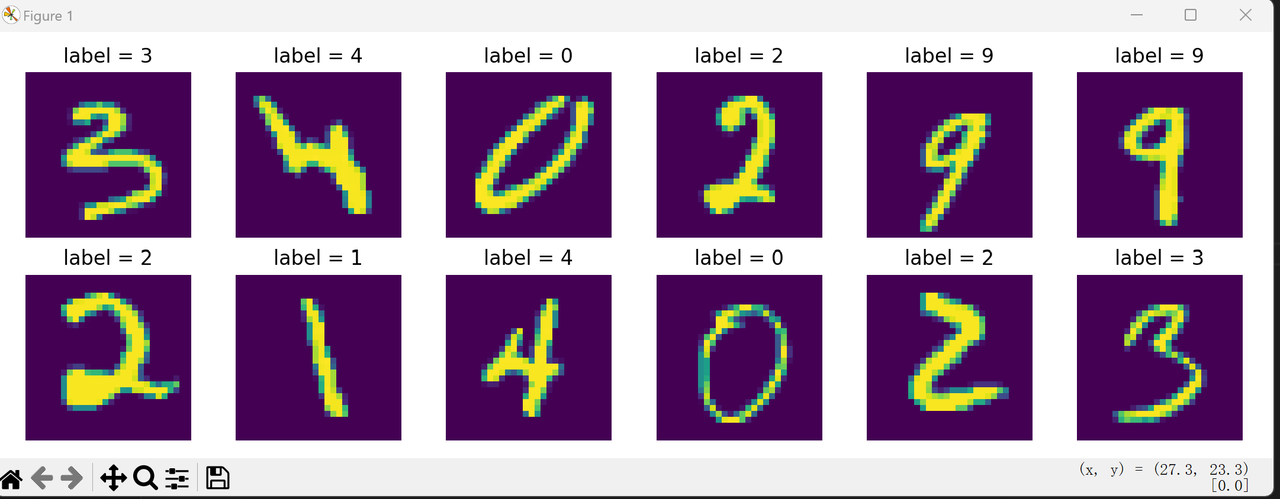
\includegraphics[width=\textwidth]{image/prob3_a_1_1.1.png}
        \caption{}
        \label{fig:second}
    \end{subfigure}
    
    \caption{Randomly chosen MNIST images with their labels.}
    \label{fig:twopics}
\end{figure}
This sanity check ensures that there are no issues with the data prior to further processing and model training.\\


\paragraph{Problem b to f}
4-layer neural network architechture satisfying (b) to (f) is shown below constructed by numpy:
\begin{lstlisting}
class embedding_t:
    """
    in:  h^l  (B,28,28)
    out: h^{l+1} (B,392) == flatten of (B,7,7,8)
    params: W (4,4,8), b (8,)
    """

    def __init__(self, seed=0):
        rs = np.random.RandomState(seed)
        # gaussian initialization
        self.w = rs.randn(4, 4, 8)
        self.b = rs.randn(8)

        # standarlize
        wnorm = np.linalg.norm(self.w.ravel())
        bnorm = np.linalg.norm(self.b)
        if wnorm > 0: self.w /= wnorm
        if bnorm > 0: self.b /= bnorm

        # gradient and cache
        self.dw = np.zeros_like(self.w)
        self.db = np.zeros_like(self.b)
        self.hl = None          # cache x
        self._patches = None    # cache patches
    
    # image <-> patch 
    def _im2patch(self, x):
        """
        x: (B,28,28) -> (B,7,7,4,4)
        """
        B = x.shape[0]
        x_reshaped = x.reshape(B, 7, 4, 7, 4)
        return x_reshaped.transpose(0, 1, 3, 2, 4)

    def _patch2im(self, patches):
        """
        (B,7,7,4,4) -> (B,28,28)
        """
        B = patches.shape[0]
        x_reshaped = patches.transpose(0, 1, 3, 2, 4)
        return x_reshaped.reshape(B, 28, 28)

    # forward
    def forward(self, h_l):
        """
        h_l: (B,28,28)
        return: h_{l+1}: (B,392)
        """
        assert h_l.ndim == 3 and h_l.shape[1:] == (28, 28)
        self.hl = h_l

        patches = self._im2patch(h_l)          
        self._patches = patches               

        h = np.einsum('bijuv, uvo -> bijo', patches, self.w)  
        h += self.b                                            

        return h.reshape(h.shape[0], -1)       

    # backward
    def backward(self, dh_next):
        # dim match
        if dh_next.ndim == 2:
            B = dh_next.shape[0]
            dh = dh_next.reshape(B, 7, 7, 8)
        else:
            dh = dh_next
            B = dh.shape[0]

        patches = self._patches  

        # gradient for b
        self.db = dh.sum(axis=(0, 1, 2))                         

        # gradient for w
        self.dw = np.einsum('bijuv, bijo -> uvo', patches, dh)   

        # gradient of patches for recursion chain rule 
        dpatches = np.einsum('bijo, uvo -> bijuv', dh, self.w)   
        dh_l = self._patch2im(dpatches)                          

        self._patches = None
        return dh_l

    def zero_grad(self):
        self.dw[...] = 0.0
        self.db[...] = 0.0

class linear_t:
    def __init__(self, in_dim=392, out_dim=10, seed=1):
        rs = np.random.RandomState(seed)
        self.w = rs.randn(out_dim, in_dim)
        self.b = rs.randn(out_dim)
        self.w /= max(np.linalg.norm(self.w), 1e-12)
        self.b /= max(np.linalg.norm(self.b), 1e-12)
        self.dw = np.zeros_like(self.w); self.db = np.zeros_like(self.b)
        self.hl = None

    def forward(self, h_l):  
        self.hl = h_l
        return h_l @ self.w.T + self.b

    def backward(self, dh_next):  
        self.dw = dh_next.T @ self.hl          
        self.db = dh_next.sum(axis=0)          
        dh_l = dh_next @ self.w                
        return dh_l

    def zero_grad(self):
        self.dw[...] = 0.0; self.db[...] = 0.0

class relu_t:
    def __init__(self):
        self.mask = None  

    def forward(self, h_l):
        self.mask = (h_l > 0)
        return np.where(self.mask, h_l, 0.0)

    def backward(self, dh_next):
        # upstream grad * 1{x>0}
        return dh_next * self.mask.astype(dh_next.dtype)

class softmax_ce_loss:
    def __init__(self):
        self.probs = None  
        self.y = None

    def forward(self, logits, y):
        """
        logits: (B, C), y: int labels (B,)
        return: scalar loss (float)
        """
        self.y = y
        z = logits - logits.max(axis=1, keepdims=True)  
        expz = np.exp(z)
        self.probs = expz / expz.sum(axis=1, keepdims=True)  

        B = logits.shape[0]
        loss = -np.log(self.probs[np.arange(B), y] + 1e-12).mean()
        return loss

    def backward(self):
        """
        dL/dlogits: (B, C)
        """
        B = self.probs.shape[0]
        dlogits = self.probs.copy()
        dlogits[np.arange(B), self.y] -= 1.0   
        dlogits /= B
        return dlogits
\end{lstlisting}

Then I verify the backward implementation by comparing analytical gradients with numerical
finite-difference estimates. Consider one hidden layer with outputs
$h^{(l)} \in \mathbb{R}^{d_l}$, weights $W \in \mathbb{R}^{d_l \times d_{l-1}}$, bias $b \in \mathbb{R}^{d_l}$,
and upstream seed $h^{(l+1)} = e_k$ (a vector with a one at entry $k$ and zeros elsewhere).
The backward function should return
\[
\text{self.dw} = \frac{\partial h^{(l+1)}_k}{\partial W},\quad
\text{self.db} = \frac{\partial h^{(l+1)}_k}{\partial b},\quad
\text{dh}^{(l)} = \frac{\partial h^{(l+1)}_k}{\partial h^{(l)}} .
\]

For any parameter entry $\theta \in \{W_{ij}, b_i, h^{(l)}_j\}$, we estimate the derivative using the
central-difference formula
\[
\frac{\partial h^{(l+1)}_k}{\partial \theta}
\approx
\frac{ \big(h^{(l)}(W+\varepsilon E)\big)_{k} - \big(h^{(l)}(W-\varepsilon E)\big)_{k} }{2\varepsilon}
\]
where $E$ is a perturbation that is zero everywhere except at the location of $\theta$,
and $\varepsilon > 0$ is small (we use $\varepsilon = 10^{-5}$).

\paragraph{Procedure.}
\begin{enumerate}
  \item Fix a random minibatch and a random index $k$ for the upstream seed $e_k$.
  \item Randomly select about ten entries of $W$ and a few entries of $b$ and $h^{(l)}$.
  \item For each selected entry $\theta$:
        form $\theta^{+}=\theta+\varepsilon$, $\theta^{-}=\theta-\varepsilon$,
        run the forward computation to obtain $h^{(l+1)}_k(\theta^{+})$ and $h^{(l+1)}_k(\theta^{-})$,
        and compute the numerical gradient by the formula above.
  \item Compare with the corresponding analytical entry from self.dw, self.db, or dh$^{(l)}$ using the
        relative error
        \[
        \text{rel\_err} =
        \frac{\lVert g_{\text{analytical}} - g_{\text{numerical}} \rVert_2}
             {\max\{1,\ \lVert g_{\text{analytical}} \rVert_2 + \lVert g_{\text{numerical}} \rVert_2\}} .
        \]
  \item Accept the implementation if the median relative error over checked entries is below $10^{-6}$
        and the maximum is below $10^{-4}$; otherwise inspect the backward formulas.
\end{enumerate}


Reference code\\
\begin{lstlisting}
def check_linear_grads(layer, in_dim=392, out_dim=10, eps=1e-5,
                       num_w_checks=10, num_b_checks=5, num_x_checks=10,
                       num_k=5, seed=0):
    rs = np.random.RandomState(seed)

    # test image input
    h_l = rs.randn(1, in_dim).astype(np.float64)
    layer.w = layer.w.astype(np.float64)
    layer.b = layer.b.astype(np.float64)

    # random k
    Ks = rs.choice(out_dim, size=min(num_k, out_dim), replace=False)

    for k in Ks:
        print(f"\n=== Checking grads for output index k={k} ===")

        # running forward/backward get gradient of h^{l+1}_k
        _ = layer.forward(h_l)                   
        dh_next = np.zeros((1, out_dim), dtype=np.float64)
        dh_next[0, k] = 1.0                      # e_k
        dh_l = layer.backward(dh_next)           

        # --------- check dW ----------
        print("Check dW (finite diff vs. backward):")
        for _ in range(num_w_checks):
            i = rs.randint(0, out_dim)          
            j = rs.randint(0, in_dim)            
            old = layer.w[i, j]

            layer.w[i, j] = old + eps
            f_pos = linear_forward_scalar_k(h_l, layer.w, layer.b, k)
            layer.w[i, j] = old - eps
            f_neg = linear_forward_scalar_k(h_l, layer.w, layer.b, k)
            layer.w[i, j] = old

            num = (f_pos - f_neg) / (2 * eps)    
            ana = layer.dw[i, j]                 
            rel_err = abs(num - ana) / max(1e-8, abs(num) + abs(ana))
            print(f"  W[{i},{j}]  num={num:+.6e}  ana={ana:+.6e}  rel_err={rel_err:.3e}")

        # --------- check db ----------
        print("Check db (finite diff vs. backward):")
        for _ in range(num_b_checks):
            i = rs.randint(0, out_dim)
            old = layer.b[i]

            layer.b[i] = old + eps
            f_pos = linear_forward_scalar_k(h_l, layer.w, layer.b, k)
            layer.b[i] = old - eps
            f_neg = linear_forward_scalar_k(h_l, layer.w, layer.b, k)
            layer.b[i] = old

            num = (f_pos - f_neg) / (2 * eps)
            ana = layer.db[i]
            rel_err = abs(num - ana) / max(1e-8, abs(num) + abs(ana))
            print(f"  b[{i}]     num={num:+.6e}  ana={ana:+.6e}  rel_err={rel_err:.3e}")

        # --------- check d h^l ----------
        print("Check d h^l (finite diff vs. backward):")
        for _ in range(num_x_checks):
            j = rs.randint(0, in_dim)
            old = h_l[0, j]

            h_l[0, j] = old + eps
            f_pos = linear_forward_scalar_k(h_l, layer.w, layer.b, k)
            h_l[0, j] = old - eps
            f_neg = linear_forward_scalar_k(h_l, layer.w, layer.b, k)
            h_l[0, j] = old

            num = (f_pos - f_neg) / (2 * eps)
            ana = dh_l[0, j]
            rel_err = abs(num - ana) / max(1e-8, abs(num) + abs(ana))
            print(f"  h_l[0,{j}] num={num:+.6e}  ana={ana:+.6e}  rel_err={rel_err:.3e}")

fc = linear_t(in_dim=392, out_dim=10, seed=1)
check_linear_grads(fc,
                   in_dim=392, out_dim=10,
                   eps=1e-5,
                   num_w_checks=10,  
                   num_b_checks=5,   
                   num_x_checks=10,  
                   num_k=5,          
                   seed=0)
\end{lstlisting}

This check is repeated for several randomly chosen entries of $W$, $b$, and $h^{(l)}$.
A close match between analytical and numerical gradients confirms the correctness
of the backward implementation. And the testing results is shown below
\begin{figure}[H]
  \centering
  \begin{subfigure}[b]{0.3\textwidth}
    \centering
    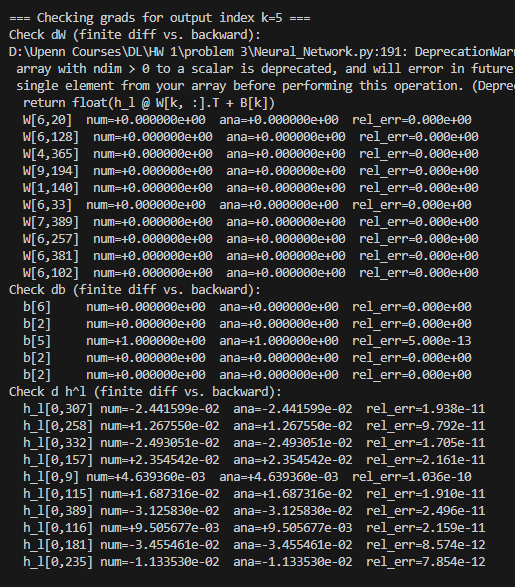
\includegraphics[width=\textwidth]{image/prob3_f_1.png}
    \caption{Result 1}\label{fig:r1}
  \end{subfigure}\hfill
  \begin{subfigure}[b]{0.3\textwidth}
    \centering
    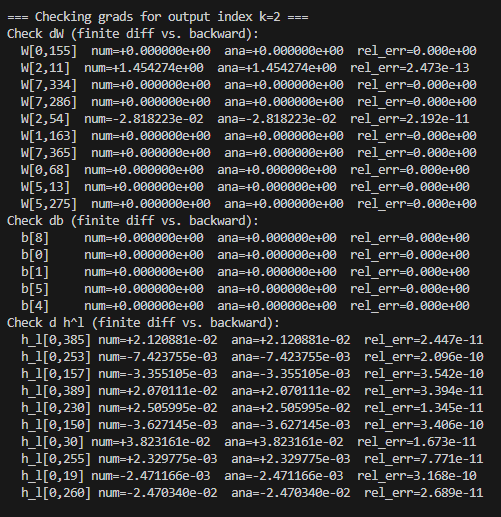
\includegraphics[width=\textwidth]{image/prob3_f_1.3.png}
    \caption{Result 2}\label{fig:r2}
  \end{subfigure}\hfill
  \begin{subfigure}[b]{0.3\textwidth}
    \centering
    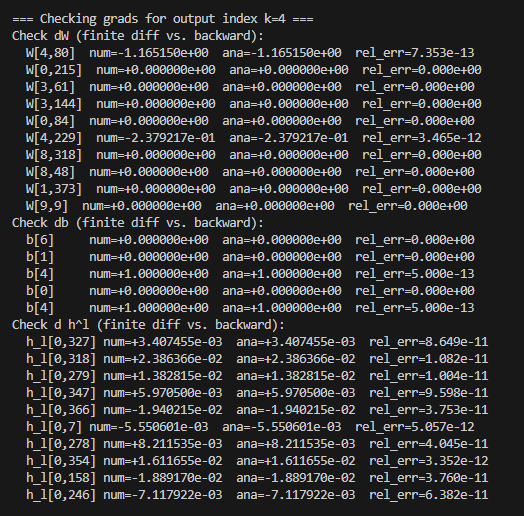
\includegraphics[width=\textwidth]{image/prob3_f_1.2.png}
    \caption{Result 3}\label{fig:r3}
  \end{subfigure}\hfill\\
  \begin{subfigure}[b]{0.3\textwidth}
    \centering
    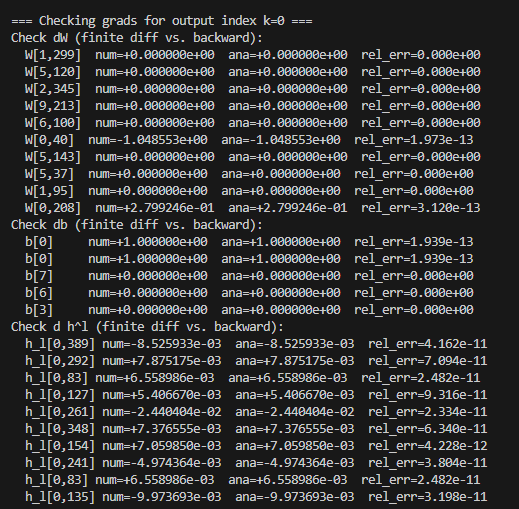
\includegraphics[width=\textwidth]{image/prob3_f_1.1.png}
    \caption{Result 4}\label{fig:r4}
  \end{subfigure}\hfill
  \begin{subfigure}[b]{0.3\textwidth}
    \centering
    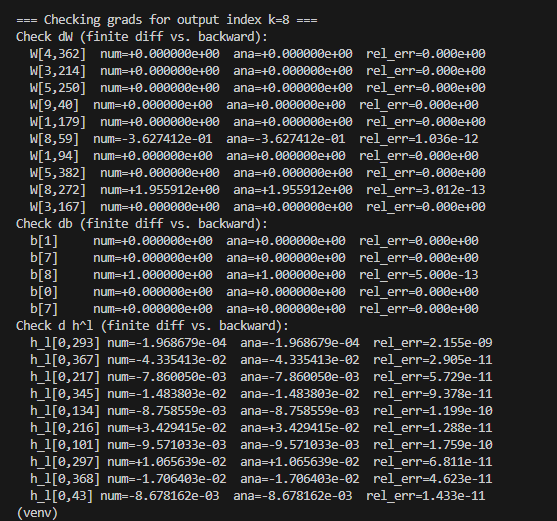
\includegraphics[width=\textwidth]{image/prob3_f_1.4.png}
    \caption{Result 5}\label{fig:r5}
  \end{subfigure}

  \caption{Five results displayed together}
  \label{fig:five-all}
\end{figure}

As illustrated in figures, the analytical and numerical gradients 
match up to machine precision. The observed relative errors are typically in the 
range $10^{-10}$ to $10^{-12}$, far below the common acceptance threshold of $10^{-6}$. 
For entries where the true gradient is zero, the numerical gradient is also zero. 
Since the analytical and numerical gradients agree within floating-point precision, 
we conclude that the backward implementation is correct.\\

\paragraph{Problem g}
It can be observed that the training loss continuously decreases as the number of training iterations increases
\begin{figure}[H]
    \centering
    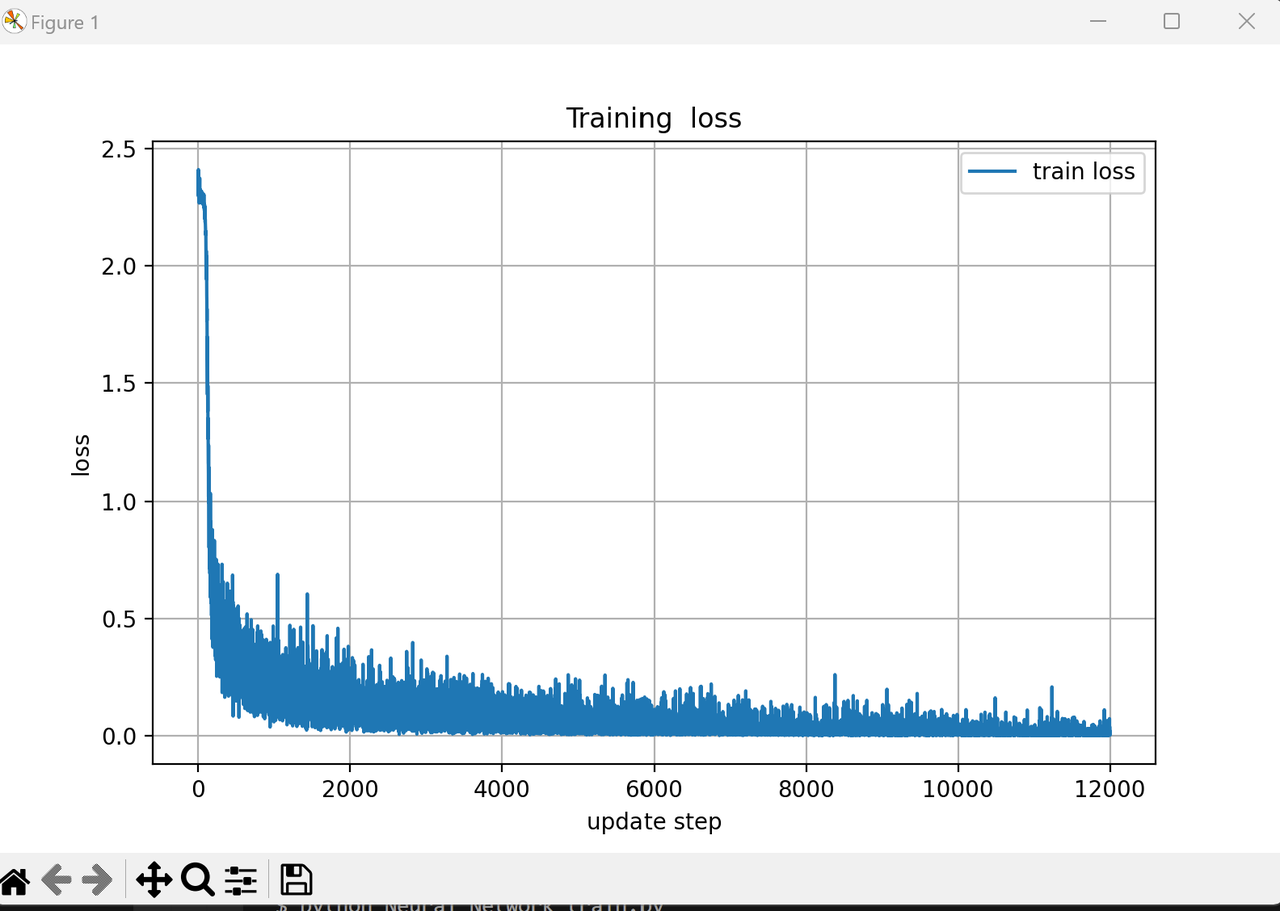
\includegraphics[width=0.8\textwidth]{image/prob3_g_1.png}
    \caption{Traning loss with epoches from 10000 to 50000}
    \label{fig:gradcheck}
\end{figure}

\paragraph{problem h}
It can be observed that the model achieves good generalization around 12,000 iterations. However, as the number of iterations increases toward 50,000, the model starts memorizing the training data, which leads to reduced generalization performance.
\begin{figure}[H]
    \centering
    \begin{subfigure}[b]{0.45\textwidth}
        \centering
        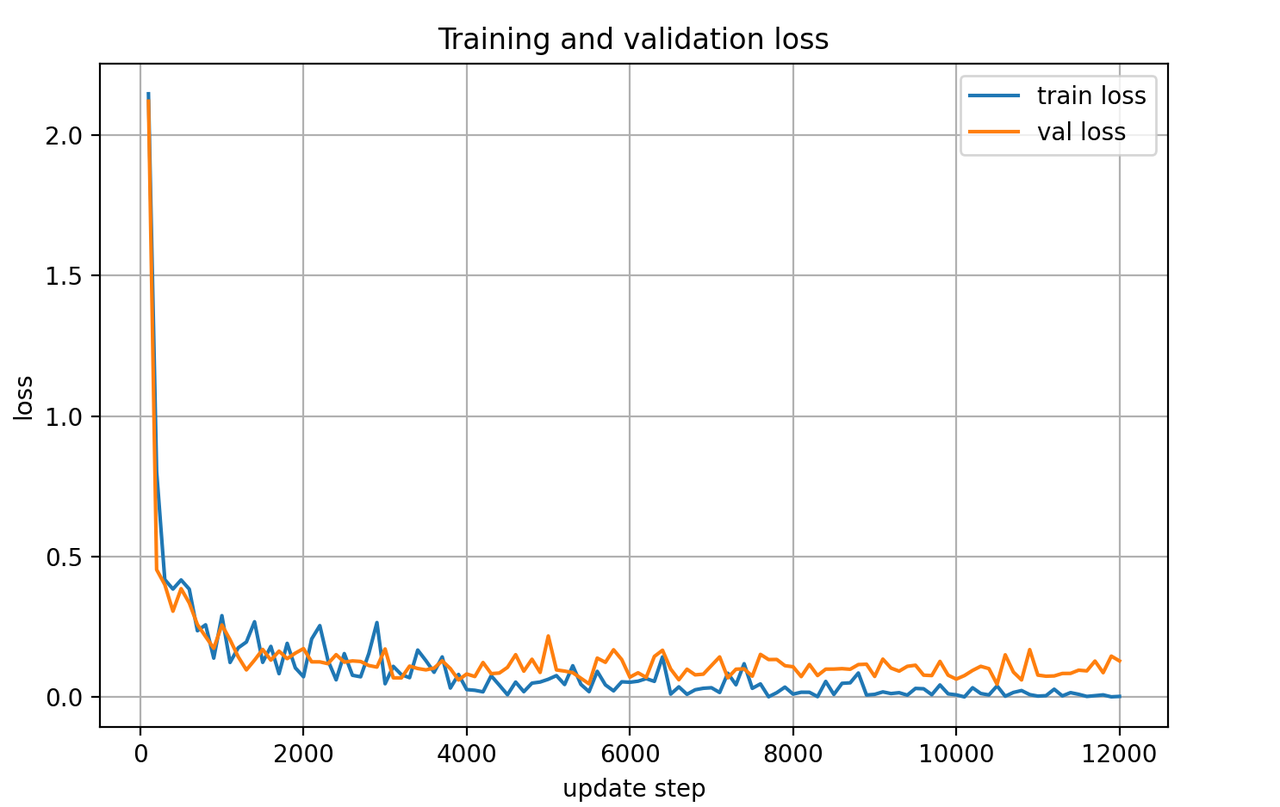
\includegraphics[width=\textwidth]{image/hprob3_h_1.png}
        \caption{}
        \label{fig:first}
    \end{subfigure}
    \hfill
    \begin{subfigure}[b]{0.45\textwidth}
        \centering
        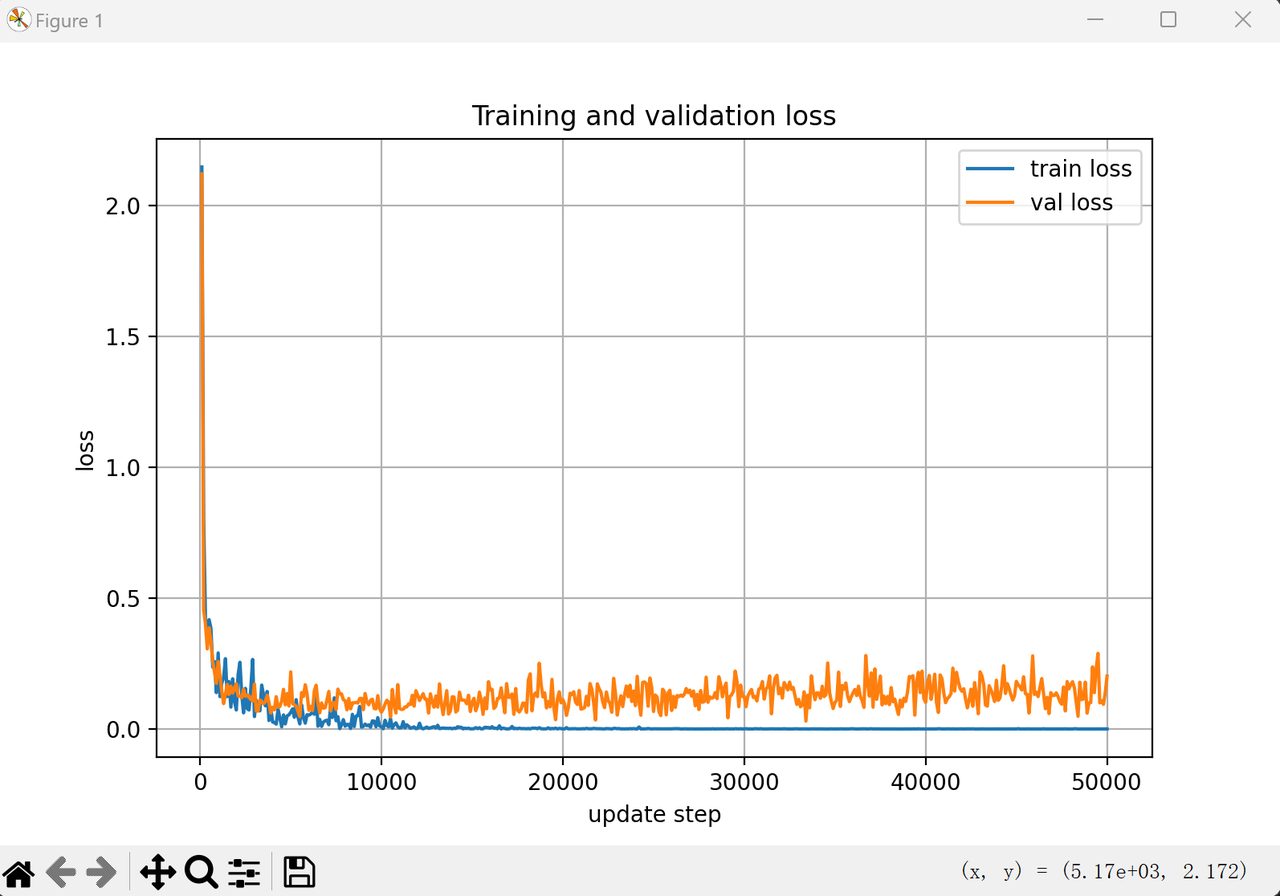
\includegraphics[width=\textwidth]{image/prob3_g_1.1.png}
        \caption{}
        \label{fig:second}
    \end{subfigure}
    
    \caption{Traning and Validation loss with itr=12000 and 10000 to 50000}
    \label{fig:twopics}
\end{figure}

\paragraph{problem i}
Similarly, it can be observed that under the PyTorch framework the results are consistent. At around 12,000 iterations the model exhibits good generalization, with the validation error slightly higher than the training error, but the training process has already converged.
\begin{figure}    
    \centering
    \begin{subfigure}[b]{0.45\textwidth}
        \centering
        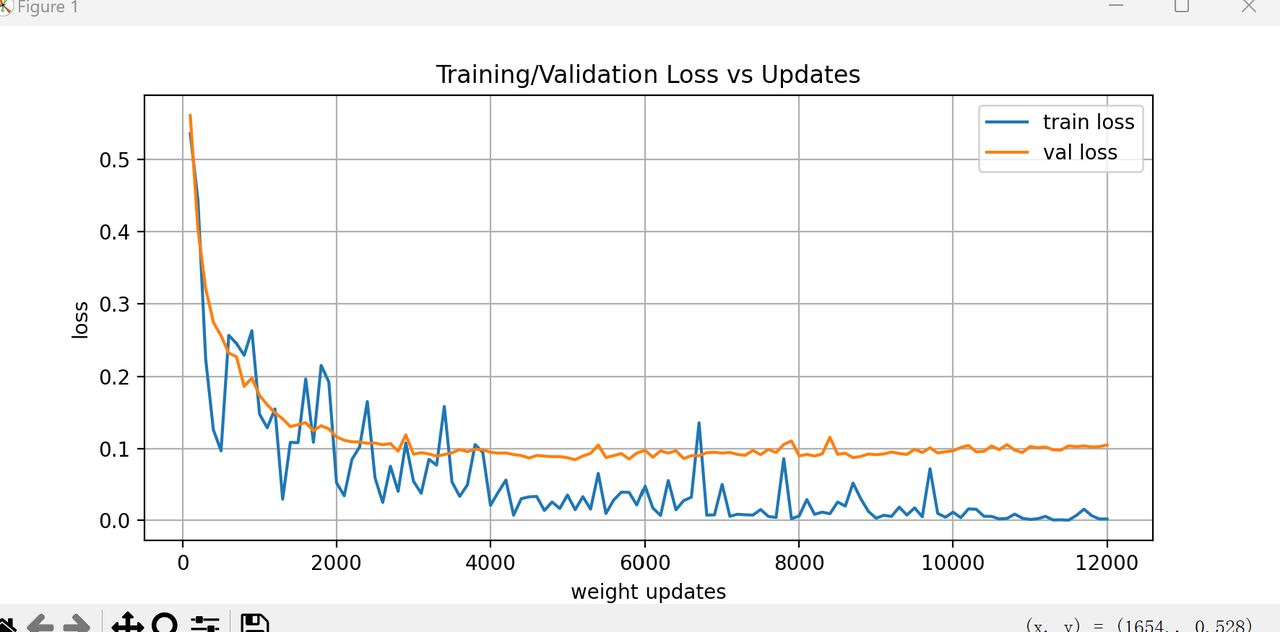
\includegraphics[width=\textwidth]{image/prob3_i_1.png}
        \caption{}
        \label{fig:first}
    \end{subfigure}
    \hfill
    \begin{subfigure}[b]{0.45\textwidth}
        \centering
        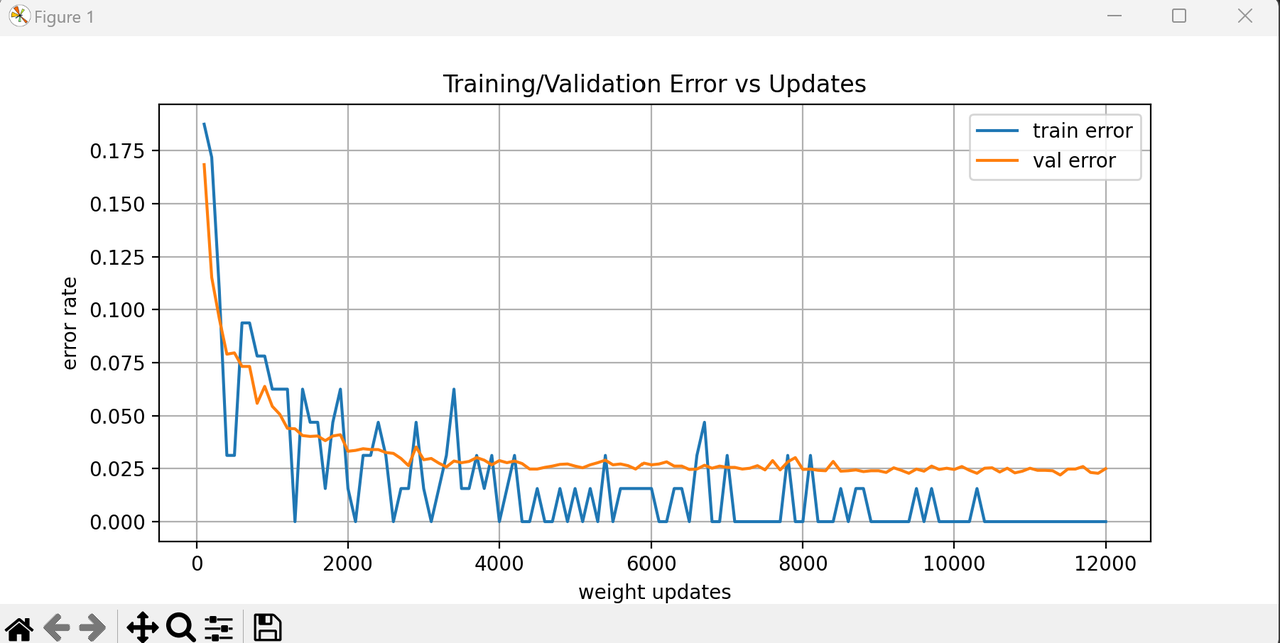
\includegraphics[width=\textwidth]{image/prob3_i_1.1.png}
        \caption{}
        \label{fig:second}
    \end{subfigure}
    
    \caption{Traning and Validation loss(error) with itr=12000 by Pytorch}
    \label{fig:twopics}
\end{figure}

\end{solution}

\appendix

\begin{lstlisting}
from sklearn.datasets import fetch_openml
from sklearn.model_selection import train_test_split, GridSearchCV
import cv2
import numpy as np
from sklearn import svm
from sklearn.metrics import accuracy_score
from sklearn.decomposition import PCA
from sklearn.preprocessing import StandardScaler

#down-sampler
def resize_14x14(im28):
        # type transform for cv2
        im28 = im28.astype(np.float32)
        return cv2.resize(im28, (14,14), interpolation=cv2.INTER_AREA)
def downsample_batch(X_flat):
    n = X_flat.shape[0]
    imgs28 = X_flat.reshape(n, 28, 28)
    imgs14 = np.stack([resize_14x14(im) for im in imgs28], axis=0)
    return imgs14.reshape(n, 14*14).astype(np.float32)

# sub-sample dataset creator
def sample_per_class(x, y, per_class=1000, random_state=42):
    rs = np.random.RandomState(random_state)
    keep_idx = []
    for digit in map(str, range(10)):
        idx = np.where(y == digit)[0]
        sel = rs.choice(idx, size=per_class, replace=False)
        keep_idx.append(sel)
    keep_idx = np.concatenate(keep_idx)
    return x[keep_idx], y[keep_idx]

# gabor fliter bank
def gabor_features_batch(x):
    # thetas = [0, np.pi/4, np.pi/2, 3*np.pi/4]
    # freqs  = [0.05, 0.20, 0.35]
    # bws    = [0.3, 0.6, 0.9]

    thetas = np.linspace(0, np.pi, 8, endpoint=False).tolist()                
    freqs  = [0.05, 0.12, 0.20, 0.28, 0.35, 0.42]                            
    bws = [3.0, 4.0, 5.0] 

    X = np.asarray(x, dtype=np.float32)
    N = X.shape[0]
    imgs = X.reshape(N, 14, 14)

    feats = []

    for th in thetas:
        for fr in freqs:
            for bw in bws:
                kernel = cv2.getGaborKernel((14, 14), sigma=4.0, theta=th,
                                            lambd=1.0/fr, gamma=0.5, psi=0,
                                            ktype=cv2.CV_32F)
                resp_list = []
                for im in imgs:
                    resp = cv2.filter2D(im, cv2.CV_32F, kernel)
                    resp_list.append(resp.ravel())
                feats.append(np.stack(resp_list, axis=0))  

    return np.concatenate(feats, axis=1).astype(np.float32)  # (N,7056)

# dataset MINIST
ds = fetch_openml('mnist_784', as_frame=False)

# Dtest/Dtrain
x_train, x_test, y_train, y_test = train_test_split(
    ds.data, ds.target, test_size=0.2, random_state=42
)
#sub-Dtest/Dtrain
x_train_sub, y_train_sub = sample_per_class(x_train, y_train, per_class=100)
x_test_sub, y_test_sub = sample_per_class(x_test, y_test, per_class=100)

x_train_sub = downsample_batch(x_train_sub)   
x_test_sub = downsample_batch(x_test_sub)

# Gabor feature generation
x_train_gabor = gabor_features_batch(x_train_sub)    
x_test_gabor = gabor_features_batch(x_test_sub)

print("Gabor feature shape:", x_train_gabor.shape)

#standarlization
scaler = StandardScaler(with_mean=True)        
x_train_std = scaler.fit_transform(x_train_gabor)
x_test_std  = scaler.transform(x_test_gabor )

#pca
pca = PCA(n_components=999, svd_solver='full', whiten=False, random_state=42)
x_train_pca = pca.fit_transform(x_train_std)
x_test_pca = pca.transform(x_test_std)

#fit svm by subDtrain
param_grid = {"C": [0.1, 0.5, 1.5, 2.5, 3, 3.5, 4, 4.5, 5, 5.5, 6]}  
base = svm.SVC(kernel='rbf', gamma='scale')

grid = GridSearchCV(
    estimator=base,
    param_grid=param_grid,
    scoring="accuracy",
    cv=5,       
    n_jobs=-1,
    refit=True,   
    verbose=3
)
grid.fit(x_train_pca, y_train_sub)

print("\n=== 5-fold CV mean accuracy for each C ===")
for mean, std, params in zip(grid.cv_results_["mean_test_score"],
                             grid.cv_results_["std_test_score"],
                             grid.cv_results_["params"]):
    print(f"{params} -> {mean:.4f} ± {std:.4f}")

print("\nBest params (by 5-fold CV):", grid.best_params_)
print("Best CV mean accuracy:", grid.best_score_)

clf = grid.best_estimator_

y_pred = clf.predict(x_test_pca)
acc = accuracy_score(y_test_sub, y_pred)
sv_ratio = len(clf.support_) / len(x_train_gabor) 

print(f"Test accuracy = {acc:.4f}")
print(f"Support vector ratio: {sv_ratio:.4f}  ({len(clf.support_)} / {len(x_train_gabor)})")
\end{lstlisting}


\begin{lstlisting}
from sklearn.datasets import fetch_openml
from sklearn.model_selection import train_test_split, GridSearchCV
import matplotlib.pyplot as plt
import cv2
import numpy as np
from sklearn import svm
from sklearn.metrics import accuracy_score, confusion_matrix
from tqdm import tqdm
  
#down-sampler
def resize_14x14(im28):
        # type transform for cv2
        im28 = im28.astype(np.float32)
        return cv2.resize(im28, (14,14), interpolation=cv2.INTER_AREA)
def downsample_batch(X_flat):
    n = X_flat.shape[0]
    imgs28 = X_flat.reshape(n, 28, 28)
    imgs14 = np.stack([resize_14x14(im) for im in imgs28], axis=0)
    return imgs14.reshape(n, 14*14).astype(np.float32)

# sub-sample dataset creator
def sample_per_class(x, y, per_class=1000, random_state=42):
    rs = np.random.RandomState(random_state)
    keep_idx = []
    for digit in map(str, range(10)):
        idx = np.where(y == digit)[0]
        sel = rs.choice(idx, size=per_class, replace=False)
        keep_idx.append(sel)
    keep_idx = np.concatenate(keep_idx)
    return x[keep_idx], y[keep_idx]

# dataset MINIST
ds = fetch_openml('mnist_784', as_frame=False)

# Dtest/Dtrain
x_train, x_test, y_train, y_test = train_test_split(
    ds.data, ds.target, test_size=0.2, random_state=42
)
#sub-Dtest/Dtrain
x_train_sub, y_train_sub = sample_per_class(x_train, y_train, per_class=1000)
x_test_sub, y_test_sub = sample_per_class(x_test, y_test, per_class=1000)

x_train_sub = downsample_batch(x_train_sub)   
x_test_sub = downsample_batch(x_test_sub) 

x_test = downsample_batch(x_test)

#fit svm by gridsearchcv to find best para.c
param_grid = {"C": [0.1, 0.5, 1.5, 2.5, 3, 3.5, 4, 4.5, 5, 5.5, 6]}  
base = svm.SVC(kernel='rbf', gamma='scale')

grid = GridSearchCV(
    estimator=base,
    param_grid=param_grid,
    scoring="accuracy",
    cv=5,       
    n_jobs=-1,
    refit=True,   
    verbose=3
)
grid.fit(x_train_sub, y_train_sub)

print("\n=== 5-fold CV mean accuracy for each C ===")
for mean, std, params in zip(grid.cv_results_["mean_test_score"],
                             grid.cv_results_["std_test_score"],
                             grid.cv_results_["params"]):
    print(f"{params} -> {mean:.4f} ± {std:.4f}")

print("\nBest params (by 5-fold CV):", grid.best_params_)
print("Best CV mean accuracy:", grid.best_score_)

# fit the model by best c
clf = grid.best_estimator_
print("\n#SV:", len(clf.support_), " / ", len(x_train_sub),
      " (ratio = {:.4f})".format(len(clf.support_) / len(x_train_sub)))

# sub test vlidation
y_test_sub_pred = clf.predict(x_test_sub)
val_acc = accuracy_score(y_test_sub, y_test_sub_pred)
val_err = 1 - val_acc
cm_sub = confusion_matrix(y_test_sub, y_test_sub_pred, labels=list(map(str, range(10))))
print("\n[Sub-Set] Validation error: {:.4f} (acc={:.4f})".format(val_err, val_acc))

# test validation
y_test_pred = clf.predict(x_test)
test_acc = accuracy_score(y_test, y_test_pred)
test_err = 1 - test_acc
cm = confusion_matrix(y_test, y_test_pred, labels=list(map(str, range(10))))
print("\n[Test] Test error: {:.4f} (acc={:.4f})".format(test_err, test_acc))
\end{lstlisting}


\begin{lstlisting}
import torchvision as thv
import numpy as np
import matplotlib.pyplot as plt

class embedding_t:
    """
    in:  h^l  (B,28,28)
    out: h^{l+1} (B,392) == flatten of (B,7,7,8)
    params: W (4,4,8), b (8,)
    """

    def __init__(self, seed=0):
        rs = np.random.RandomState(seed)
        # gaussian initialization
        self.w = rs.randn(4, 4, 8)
        self.b = rs.randn(8)

        # standarlize
        wnorm = np.linalg.norm(self.w.ravel())
        bnorm = np.linalg.norm(self.b)
        if wnorm > 0: self.w /= wnorm
        if bnorm > 0: self.b /= bnorm

        # gradient and cache
        self.dw = np.zeros_like(self.w)
        self.db = np.zeros_like(self.b)
        self.hl = None          # cache x
        self._patches = None    # cache patches
    
    # image <-> patch 
    def _im2patch(self, x):
        """
        x: (B,28,28) -> (B,7,7,4,4)
        """
        B = x.shape[0]
        x_reshaped = x.reshape(B, 7, 4, 7, 4)
        return x_reshaped.transpose(0, 1, 3, 2, 4)

    def _patch2im(self, patches):
        """
        (B,7,7,4,4) -> (B,28,28)
        """
        B = patches.shape[0]
        x_reshaped = patches.transpose(0, 1, 3, 2, 4)
        return x_reshaped.reshape(B, 28, 28)

    # forward
    def forward(self, h_l):
        """
        h_l: (B,28,28)
        return: h_{l+1}: (B,392)
        """
        assert h_l.ndim == 3 and h_l.shape[1:] == (28, 28)
        self.hl = h_l

        patches = self._im2patch(h_l)          
        self._patches = patches               

        h = np.einsum('bijuv, uvo -> bijo', patches, self.w)  
        h += self.b                                            

        return h.reshape(h.shape[0], -1)       

    # backward
    def backward(self, dh_next):
        # dim match
        if dh_next.ndim == 2:
            B = dh_next.shape[0]
            dh = dh_next.reshape(B, 7, 7, 8)
        else:
            dh = dh_next
            B = dh.shape[0]

        patches = self._patches  

        # gradient for b
        self.db = dh.sum(axis=(0, 1, 2))                         

        # gradient for w
        self.dw = np.einsum('bijuv, bijo -> uvo', patches, dh)   

        # gradient of patches for recursion chain rule 
        dpatches = np.einsum('bijo, uvo -> bijuv', dh, self.w)   
        dh_l = self._patch2im(dpatches)                          

        self._patches = None
        return dh_l

    def zero_grad(self):
        self.dw[...] = 0.0
        self.db[...] = 0.0

class linear_t:
    def __init__(self, in_dim=392, out_dim=10, seed=1):
        rs = np.random.RandomState(seed)
        self.w = rs.randn(out_dim, in_dim)
        self.b = rs.randn(out_dim)
        self.w /= max(np.linalg.norm(self.w), 1e-12)
        self.b /= max(np.linalg.norm(self.b), 1e-12)
        self.dw = np.zeros_like(self.w); self.db = np.zeros_like(self.b)
        self.hl = None

    def forward(self, h_l):  
        self.hl = h_l
        return h_l @ self.w.T + self.b

    def backward(self, dh_next):  
        self.dw = dh_next.T @ self.hl          
        self.db = dh_next.sum(axis=0)          
        dh_l = dh_next @ self.w                
        return dh_l

    def zero_grad(self):
        self.dw[...] = 0.0; self.db[...] = 0.0

class relu_t:
    def __init__(self):
        self.mask = None  

    def forward(self, h_l):
        self.mask = (h_l > 0)
        return np.where(self.mask, h_l, 0.0)

    def backward(self, dh_next):
        # upstream grad * 1{x>0}
        return dh_next * self.mask.astype(dh_next.dtype)

class softmax_ce_loss:
    def __init__(self):
        self.probs = None  
        self.y = None

    def forward(self, logits, y):
        """
        logits: (B, C), y: int labels (B,)
        return: scalar loss (float)
        """
        self.y = y
        z = logits - logits.max(axis=1, keepdims=True)  
        expz = np.exp(z)
        self.probs = expz / expz.sum(axis=1, keepdims=True)  

        B = logits.shape[0]
        loss = -np.log(self.probs[np.arange(B), y] + 1e-12).mean()
        return loss

    def backward(self):
        """
        dL/dlogits: (B, C)
        """
        B = self.probs.shape[0]
        dlogits = self.probs.copy()
        dlogits[np.arange(B), self.y] -= 1.0   
        dlogits /= B
        return dlogits

class SimpleMNISTModel:
    def __init__(self):
        self.embed = embedding_t()
        self.fc1   = linear_t(in_dim=392, out_dim=128) 
        self.relu  = relu_t()
        self.fc2   = linear_t(in_dim=128, out_dim=10)
        self.lossf = softmax_ce_loss()

    def zero_grad(self):
        self.embed.zero_grad()
        self.fc1.zero_grad()
        self.fc2.zero_grad()

    def forward(self, x):             
        h  = self.embed.forward(x)    
        z1 = self.fc1.forward(h)      
        a1 = self.relu.forward(z1)    
        logits = self.fc2.forward(a1) 
        return logits

    def backward(self, dlogits):
        da1 = self.fc2.backward(dlogits)   
        dz1 = self.relu.backward(da1)      
        dh  = self.fc1.backward(dz1)       
        _   = self.embed.backward(dh)      

    def step(self, lr=0.1):
        # SGD 
        self.embed.w -= lr * self.embed.dw; self.embed.b -= lr * self.embed.db
        self.fc1.w   -= lr * self.fc1.dw;   self.fc1.b   -= lr * self.fc1.db
        self.fc2.w   -= lr * self.fc2.dw;   self.fc2.b   -= lr * self.fc2.db

def validate(model, x_val, y_val, batch_size=32):
  
    N = len(y_val)
    total_loss = 0.0
    total_correct = 0

    # sequential
    for i in range(0, N, batch_size):
        xb = x_val[i:i+batch_size]
        yb = y_val[i:i+batch_size]

        logits = model.forward(xb)          
        loss = model.lossf.forward(logits, yb)
        total_loss += loss * len(yb)
        preds = np.argmax(logits, axis=1)
        total_correct += np.sum(preds == yb)

    avg_loss = total_loss / N
    avg_error = 1.0 - (total_correct / N)
    return avg_loss, avg_error



# Take 50% from EACH CLASS (stratified)
def stratified_half(x, y, rng=42):
    rs = np.random.RandomState(rng)
    keep_idx = []
    for c in range(10):  
        idx_c = np.where(y == c)[0]
        rs.shuffle(idx_c)
        k = len(idx_c) // 2  
        keep_idx.append(idx_c[:k])
    keep_idx = np.concatenate(keep_idx)
    rs.shuffle(keep_idx)
    return x[keep_idx], y[keep_idx]

train = thv.datasets.MNIST("./", download=True, train=True)
val   = thv.datasets.MNIST("./", download=True, train=False)
#print("Raw:", train.data.shape, len(train.targets), "|", val.data.shape, len(val.targets))

# Convert to NumPy instead of torch tensor
x_tr = train.data.numpy()      
y_tr = train.targets.numpy()   
x_va = val.data.numpy()        
y_va = val.targets.numpy()

x_tr_sub, y_tr_sub = stratified_half(x_tr, y_tr, rng=123)
x_va_sub, y_va_sub = stratified_half(x_va, y_va, rng=456)

# x: (N,28,28) uint8 -> float32 in [0,1]
x_tr_sub = (x_tr_sub.astype(np.float32) / 255.0)
x_va_sub = (x_va_sub.astype(np.float32) / 255.0)
y_tr_sub = y_tr_sub.astype(np.int64)
y_va_sub = y_va_sub.astype(np.int64)

# training loop
def batch_iter(X, Y, bs, rng):
    n = len(Y)
    idx = rng.choice(n, size=bs, replace=False)
    return X[idx], Y[idx]

def accuracy(logits, y):
    return np.mean(np.argmax(logits, axis=1) == y)

rng = np.random.RandomState(0)
model = SimpleMNISTModel()
lr = 0.1
batch_size = 64
updates = 50000   # steps

val_steps = []
val_losses = []
val_errors = []

for t in range(1, updates+1):
    xb, yb = batch_iter(x_tr_sub, y_tr_sub, batch_size, rng)

    model.zero_grad()
    logits = model.forward(xb)
    loss = model.lossf.forward(logits, yb)
    dlogits = model.lossf.backward()
    model.backward(dlogits)
    model.step(lr)

    if t % 1000 == 0:
        vloss, verr = validate(model, x_va_sub, y_va_sub, batch_size=32)
        val_steps.append(t)
        val_losses.append(vloss)
        val_errors.append(verr)
        print(f"[val @ {t}] loss={vloss:.4f}, error={verr:.3f}")

plt.figure(figsize=(8,4))
plt.plot(val_steps, val_losses, marker='o', label='val loss')
plt.xlabel('weight updates')
plt.ylabel('loss')
plt.title('Validation loss vs updates (every 1000)')
plt.grid(True); plt.legend()
plt.show()

plt.figure(figsize=(8,4))
plt.plot(val_steps, val_errors, marker='o', label='val error')
plt.xlabel('weight updates')
plt.ylabel('error rate')
plt.title('Validation error vs updates (every 1000)')
plt.grid(True); plt.legend()
plt.show()    
\end{lstlisting}


\begin{lstlisting}
import torch
import torch.nn as nn
import torchvision as thv
from torch.utils.data import TensorDataset, DataLoader
import numpy as np
import matplotlib.pyplot as plt

# reproducibility & device
seed = 0
torch.manual_seed(seed); np.random.seed(seed)
device = torch.device("cuda" if torch.cuda.is_available() else "cpu")
print("device:", device)

# Dataset
root = "./"
train = thv.datasets.MNIST(root, download=True, train=True)
val   = thv.datasets.MNIST(root, download=True, train=False)

def stratified_half_indices(targets: np.ndarray, rng=42):
    rs = np.random.RandomState(rng)
    keep = []
    for c in range(10):
        idx = np.where(targets == c)[0]
        rs.shuffle(idx)
        keep.append(idx[:len(idx)//2])
    keep = np.concatenate(keep)
    rs.shuffle(keep)
    return keep

x_tr = train.data.numpy().astype(np.float32)/255.0
y_tr = train.targets.numpy().astype(np.int64)
x_va = val.data.numpy().astype(np.float32)/255.0
y_va = val.targets.numpy().astype(np.int64)

tr_idx = stratified_half_indices(y_tr, rng=123)
va_idx = stratified_half_indices(y_va, rng=456)

x_tr_t = torch.from_numpy(x_tr[tr_idx]).unsqueeze(1)  
y_tr_t = torch.from_numpy(y_tr[tr_idx])
x_va_t = torch.from_numpy(x_va[va_idx]).unsqueeze(1)
y_va_t = torch.from_numpy(y_va[va_idx])

train_ds = TensorDataset(x_tr_t, y_tr_t)
val_ds   = TensorDataset(x_va_t, y_va_t)

# DataLoader 
val_loader = DataLoader(val_ds, batch_size=256, shuffle=False)


# Model with 4 layers
class SimpleMNISTModel(nn.Module):
    def __init__(self):
        super().__init__()
        self.embed = nn.Conv2d(1, 8, kernel_size=4, stride=4, bias=True)  
        self.fc1   = nn.Linear(8*7*7, 128)
        self.relu  = nn.ReLU()
        self.fc2   = nn.Linear(128, 10)

    def forward(self, x):
        h = self.embed(x)         
        h = h.flatten(1)   
        # model       
        h = self.relu(self.fc1(h))
        return self.fc2(h)        

@torch.no_grad()
def evaluate(model, loader, lossf):
    model.eval()
    total_loss, total_correct, total = 0.0, 0, 0
    for xb, yb in loader:
        xb, yb = xb.to(device), yb.to(device)
        logits = model(xb)
        loss = lossf(logits, yb)
        total_loss += loss.item()*yb.size(0)
        total_correct += (logits.argmax(1)==yb).sum().item()
        total += yb.size(0)
    return total_loss/total, 1.0 - total_correct/total  # (loss, error)


# Training config
model = SimpleMNISTModel().to(device)
optimizer = torch.optim.SGD(model.parameters(), lr=0.1)
lossf = nn.CrossEntropyLoss()

batch_size = 64
updates = 12000             
eval_every = 100          

rng = np.random.RandomState(0)
def sample_batch(ds, bs):
    n = len(ds)
    idx = rng.choice(n, size=bs, replace=False)
    return ds.tensors[0][idx], ds.tensors[1][idx]

# Train
steps = []
train_losses, train_errors = [], []
val_losses,   val_errors   = [], []

for t in range(1, updates+1):
    model.train()
    xb, yb = sample_batch(train_ds, batch_size)
    xb, yb = xb.to(device), yb.to(device)

    optimizer.zero_grad(set_to_none=True)
    logits = model(xb)
    loss = lossf(logits, yb)
    loss.backward()
    optimizer.step()

    if t % eval_every == 0:
        # training metrics
        with torch.no_grad():
            preds = logits.argmax(1)
            train_err = 1.0 - (preds==yb).float().mean().item()
            train_loss = loss.item()

        # validation metrics
        vloss, verr = evaluate(model, val_loader, lossf)

        steps.append(t)
        train_losses.append(train_loss); train_errors.append(train_err)
        val_losses.append(vloss);        val_errors.append(verr)

        print(f"[{t:5d}] train_loss={train_loss:.4f} train_err={train_err:.3f} | "
              f"val_loss={vloss:.4f} val_err={verr:.3f}")


# Plots
plt.figure(figsize=(9,4))
plt.plot(steps, train_losses, label='train loss')
plt.plot(steps, val_losses, label='val loss')
plt.xlabel('weight updates'); plt.ylabel('loss')
plt.title('Training/Validation Loss vs Updates')
plt.grid(True); plt.legend()
plt.show()

plt.figure(figsize=(9,4))
plt.plot(steps, train_errors, label='train error')
plt.plot(steps, val_errors, label='val error')
plt.xlabel('weight updates'); plt.ylabel('error rate')
plt.title('Training/Validation Error vs Updates')
plt.grid(True); plt.legend()
plt.show()
\end{lstlisting}
\end{document}
